% !TeX program = xelatex
\documentclass[UTF8,a4paper,12pt]{ctexart}

\usepackage{geometry}
\geometry{left=2.6cm,right=2.6cm,top=2.5cm,bottom=2.5cm}
\usepackage{amsmath,amssymb,bm}
\usepackage{booktabs,multirow}
\usepackage{graphicx}
\usepackage{subcaption}
\usepackage{float}
\usepackage{xcolor}
\usepackage{hyperref}
\usepackage{listings}
\usepackage{enumitem}
\usepackage{siunitx}
\usepackage{fancyhdr}

\hypersetup{colorlinks=true,linkcolor=blue!55!black,urlcolor=blue!55!black}
\graphicspath{{results/complete/}{results/complete/models/}{results/complete/snr/}}
\setlength{\parindent}{2em}
\setlength{\parskip}{0.25em}
\linespread{1.25}
\sisetup{round-mode=places,round-precision=2}

\pagestyle{fancy}
\setlength{\headheight}{15pt}
\fancyhf{}
\fancyhead[L]{MIMO--OFDM CSI 信道估计实验报告}
\fancyhead[R]{\thepage}
\renewcommand{\headrulewidth}{0.4pt}

\lstset{
  basicstyle=\ttfamily\small,
  backgroundcolor=\color{gray!8},
  frame=single,
  breaklines=true,
  columns=fullflexible
}

% 请在提交前填写以下信息
\newcommand{\studentclass}{2023211119}
\newcommand{\studentname}{李星昱}
\newcommand{\studentid}{2023212207}
\newcommand{\coursename}{无线通信中的人工智能}

\begin{document}

\begin{titlepage}
  \centering
  \vspace*{2.0cm}
  {\zihao{1}\bfseries MIMO--OFDM 系统 CSI 信道估计实验报告\par}
  \vspace{0.8cm}
  {\zihao{3} 基于 LS、LMMSE 与深度残差网络的对比研究\par}
  \vfill
  \renewcommand{\arraystretch}{1.8}
  \begin{tabular}{rl}
    课程名称： & \coursename \\
    班\hspace{2em}级： & \studentclass \\
    学生姓名： & \studentname \\
    学\hspace{2em}号： & \studentid \\
    实验日期： & 2026 年 6 月 27 日 \\
  \end{tabular}
  \vfill
  {\large \today\par}
\end{titlepage}

\pagenumbering{Roman}
\begin{abstract}
本实验面向频率选择性 $4\times4$ MIMO--OFDM 系统，研究已知正交导频条件下的信道状态信息（Channel State Information, CSI）估计。实验基于物理一致的接收模型 $\bm Y=\bm H\bm X+\bm N$ 构造独立 Rayleigh 信道与具有空频相关性的多径信道，比较最小二乘（LS）、标量线性最小均方误差（LMMSE）以及残差 CNN、LSTM 和 Transformer 估计器。默认配置包含 32 个子载波、6 条时域径、$0$--$30$ dB 随机信噪比，训练集、验证集和测试集分别为 10000、2000 和 3000 个独立样本。

结果表明：在固定 SNR 扫描中，CNN 在 $0$--$25$ dB 区间始终优于 LS 与标量 LMMSE，在 10 dB 时获得 $-16.00$ dB NMSE，相对 LMMSE 改善约 5.62 dB；随着 SNR 提高到 30 dB，三者差距收窄。在混合 SNR 的架构对比实验中，Transformer 达到最低总体 NMSE（$-16.30$ dB），CNN 以约 $7.5\%$ 的参数量获得 $-15.33$ dB，体现出较好的精度--复杂度折中。进一步的信道消融显示，在独立 Rayleigh 信道上三类神经网络均未超过 LMMSE，而在相关多径信道上均获得明显增益。新增提高实验中，扩大 CNN 至 505,538 个参数仅改善 0.067 dB；引入有限时延投影的 Physics-Guided CNN 则达到 $-17.14$ dB，相对原始 CNN 提高 2.22 dB，证明物理先验比单纯增加网络容量更加有效。

\noindent\textbf{关键词：} MIMO--OFDM；信道估计；CSI；LMMSE；卷积神经网络；Transformer；NMSE
\end{abstract}

\tableofcontents
\listoffigures
\clearpage
\pagenumbering{arabic}

\section{实验目的}

本实验的主要目标如下：
\begin{enumerate}[label=(\arabic*)]
  \item 建立具有正交导频、加性高斯白噪声和频率选择性衰落的 MIMO--OFDM 信道仿真链路；
  \item 实现 LS 与标量 LMMSE 两类传统基线，并实现 CNN、LSTM、Transformer 三类残差式神经估计器；
  \item 定量分析估计性能随 SNR 的变化规律，比较不同深度模型的精度、收敛特性与参数规模；
  \item 对比独立 Rayleigh 与相关多径信道，判断神经网络性能增益的来源；
  \item 通过信道幅度热力图与残差分布验证定量指标所反映的估计质量。
\end{enumerate}

\section{系统模型与评价指标}

\subsection{MIMO--OFDM 导频观测模型}

系统包含 $N_r=4$ 根接收天线、$N_t=4$ 根发送天线和 $K=32$ 个子载波。在第 $k$ 个子载波上，接收导频矩阵表示为
\begin{equation}
  \bm Y_k=\bm H_k\bm X+\bm N_k,
  \label{eq:system}
\end{equation}
其中，$\bm H_k\in\mathbb C^{N_r\times N_t}$ 为真实频域信道，$\bm X\in\mathbb C^{N_t\times N_t}$ 为单位化 DFT 正交导频，满足 $\bm X\bm X^{\mathrm H}=\bm I$，$\bm N_k$ 为复高斯白噪声。每个样本的信噪比在指定区间内均匀抽取，噪声方差由接收信号功率计算：
\begin{equation}
  \sigma_n^2=\frac{P_y}{10^{\mathrm{SNR}/10}}.
\end{equation}

\subsection{信道模型}

实验使用两种合成信道。

\textbf{独立 Rayleigh 信道：} 不同收发天线与子载波上的系数相互独立，且
\begin{equation}
  H_{r,t,k}\sim\mathcal{CN}(0,1).
\end{equation}

\textbf{相关多径信道：} 首先生成 $L=6$ 条复高斯时域径，其功率按指数规律衰减并归一化；随后利用指数型相关矩阵
\begin{equation}
  [\bm R]_{i,j}=\rho^{|i-j|},\qquad \rho=0.6
\end{equation}
在收发两端引入空间相关性，最后沿时延维进行 32 点 FFT 得到频域信道。该模型同时包含邻近天线与邻近子载波间的可学习结构。

\subsection{传统估计器}

由导频的酉正交性质，LS 估计为
\begin{equation}
  \widehat{\bm H}_{\mathrm{LS},k}=\bm Y_k\bm X^{\mathrm H}.
\end{equation}
实验中的 LMMSE 是基于单位信道方差的标量收缩基线，而非使用完整信道协方差矩阵的矩阵 LMMSE：
\begin{equation}
  \widehat{\bm H}_{\mathrm{LMMSE},k}
  =\frac{\sigma_h^2}{\sigma_h^2+\sigma_n^2}
  \widehat{\bm H}_{\mathrm{LS},k},\qquad \sigma_h^2=1.
  \label{eq:lmmse}
\end{equation}

\subsection{深度残差估计器}

三种网络均以 LS 估计和对数噪声方差为输入，学习估计误差的残差：
\begin{equation}
  \widehat{\bm H}_{\theta}
  =\widehat{\bm H}_{\mathrm{LS}}+
  f_{\theta}\!\left(\widehat{\bm H}_{\mathrm{LS}},\log_{10}\sigma_n^2\right).
\end{equation}
复数信道被拆分为实部与虚部两个通道。

\begin{itemize}
  \item \textbf{CNN：} 使用三维卷积联合处理实虚部、收发天线和子载波维度，隐藏通道数为 32；
  \item \textbf{LSTM：} 将每个子载波的 $4\times4$ 复信道展平为序列特征，采用两层、隐藏维度 128 的 LSTM；
  \item \textbf{Transformer：} 采用维度 128 的线性嵌入、正弦位置编码和两层四头 Transformer Encoder。
\end{itemize}

训练损失为批内样本 NMSE 的平均值。对预测 $\widehat{\bm H}$，归一化均方误差定义为
\begin{equation}
  \mathrm{NMSE}=\frac{\lVert\widehat{\bm H}-\bm H\rVert_F^2}
  {\lVert\bm H\rVert_F^2},\qquad
  \mathrm{NMSE}_{\mathrm{dB}}=10\log_{10}(\mathrm{NMSE}).
  \label{eq:nmse}
\end{equation}
因此，NMSE 的 dB 数值越低（越负），估计性能越好。

\section{实验设置}

所有数据均由程序在线合成，不使用外部实测数据。训练、验证和测试集采用不同随机种子生成，从数据源头避免样本泄漏。默认实验参数见表~\ref{tab:settings}。

\begin{table}[H]
  \centering
  \caption{默认实验配置}
  \label{tab:settings}
  \begin{tabular}{lc@{\hspace{1.2cm}}lc}
    \toprule
    参数 & 取值 & 参数 & 取值 \\
    \midrule
    收发天线数 & $4\times4$ & 子载波数 & 32 \\
    多径数 & 6 & 空间相关系数 & 0.6 \\
    训练/验证/测试样本 & 10000/2000/3000 & SNR 范围 & 0--30 dB \\
    主架构实验训练轮数 & 20 & 场景图矩阵训练轮数 & 12 \\
    批大小 & 128 & 优化器 & Adam \\
    初始学习率 & $10^{-3}$ & 随机种子 & 2026 \\
    主评价指标 & NMSE (dB) & 数据来源 & 程序合成 \\
    \bottomrule
  \end{tabular}
\end{table}

实验包含三组核心对比：第一组在 0、5、10、15、20、25、30 dB 固定 SNR 测试集上比较 LS、LMMSE 和 CNN；第二组在 $0$--$30$ dB 混合 SNR 多径数据上比较三种网络；第三组分别在独立 Rayleigh 和相关多径信道上重新训练并评价三种网络，以分析信道结构的影响。

\section{实验结果与分析}

\subsection{不同 SNR 下的估计性能}

固定 SNR 测试结果见表~\ref{tab:snr} 与图~\ref{fig:snr}。

\begin{table}[H]
  \centering
  \caption{不同 SNR 下各估计器的 NMSE（dB，越低越好）}
  \label{tab:snr}
  \begin{tabular}{rrrrr}
    \toprule
    SNR (dB) & LS & LMMSE & CNN & CNN 相对 LMMSE 改善 \\
    \midrule
     0 &  $-0.01$ &  $-2.93$ &  $-7.95$ & 5.02 \\
     5 &  $-5.00$ &  $-6.14$ & $-11.84$ & 5.71 \\
    10 &  $-9.99$ & $-10.38$ & $-16.00$ & 5.62 \\
    15 & $-15.00$ & $-15.13$ & $-20.17$ & 5.04 \\
    20 & $-20.00$ & $-20.04$ & $-24.14$ & 4.11 \\
    25 & $-25.01$ & $-25.02$ & $-27.61$ & 2.60 \\
    30 & $-30.00$ & $-30.01$ & $-29.88$ & $-0.12$ \\
    \bottomrule
  \end{tabular}
\end{table}

\begin{figure}[H]
  \centering
  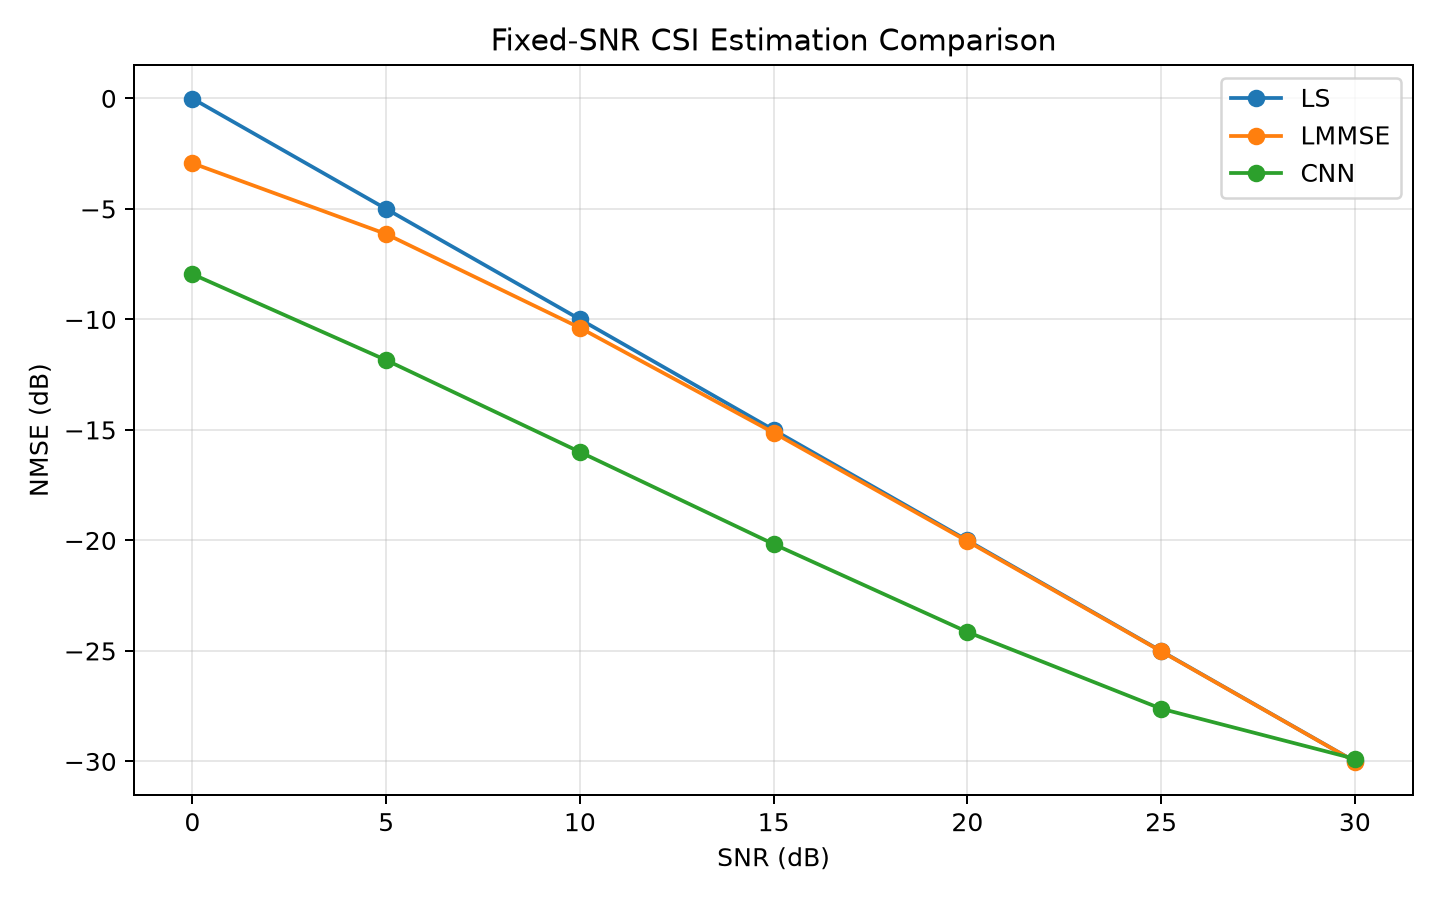
\includegraphics[width=0.88\textwidth]{fixed_snr_comparison.png}
  \caption{LS、标量 LMMSE 与 CNN 的固定 SNR 性能对比}
  \label{fig:snr}
\end{figure}

LS 曲线近似随 SNR 以 $-1$ dB/dB 的斜率下降，说明仿真链路中的噪声标定正确。LMMSE 在低 SNR 区间通过收缩抑制噪声，0 dB 时较 LS 改善约 2.93 dB；在高 SNR 下收缩系数趋近 1，因此逐渐退化为 LS。CNN 在 0--25 dB 区间表现最佳，其中 5--15 dB 的优势约为 5--6 dB。这说明网络能利用相关多径信道的局部空频结构完成超越逐元素收缩的去噪。30 dB 时，噪声已很弱，而网络仍存在有限逼近误差，因而与解析基线基本持平且略差 0.12 dB。

\subsection{CNN、LSTM 与 Transformer 架构对比}

在相同多径数据与训练配置下，三类模型的总体测试结果见表~\ref{tab:models}。

\begin{table}[H]
  \centering
  \caption{深度模型总体性能与参数规模}
  \label{tab:models}
  \begin{tabular}{lrrrr}
    \toprule
    模型 & NMSE (dB) & 相对 LMMSE 改善 (dB) & 参数量 & 最优验证 NMSE \\
    \midrule
    CNN & $-15.33$ & 5.44 & 30,370 & 0.02894 \\
    LSTM & $-13.59$ & 3.70 & 219,680 & 0.04328 \\
    Transformer & $\mathbf{-16.30}$ & $\mathbf{6.41}$ & 405,024 & $\mathbf{0.02324}$ \\
    \midrule
    LS 基线 & $-8.34$ & --- & --- & --- \\
    LMMSE 基线 & $-9.89$ & --- & --- & --- \\
    \bottomrule
  \end{tabular}
\end{table}

\begin{figure}[H]
  \centering
  \begin{subfigure}[t]{0.49\textwidth}
    \centering
    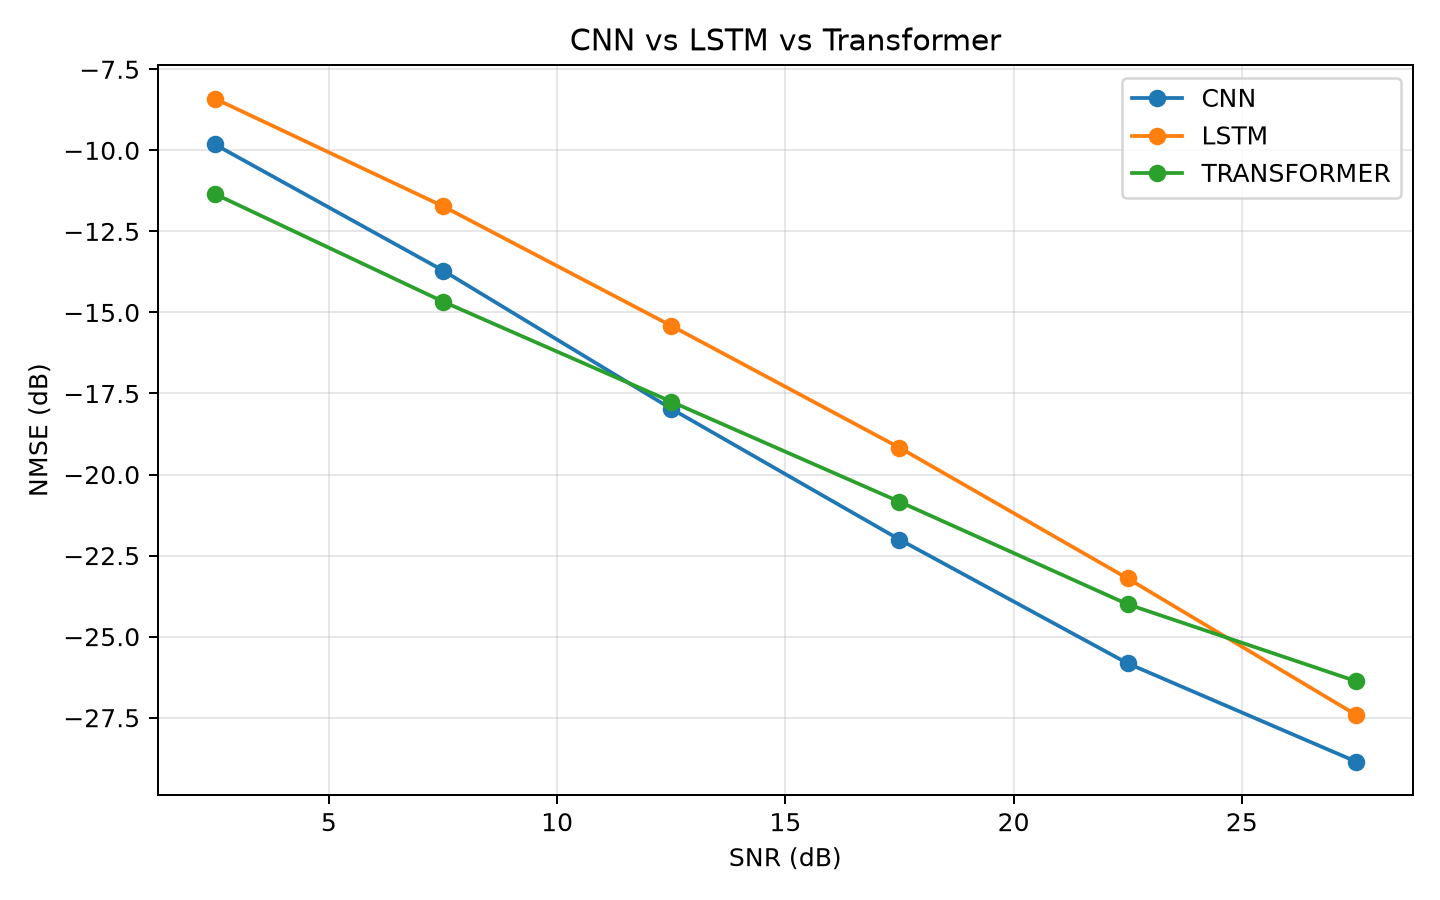
\includegraphics[width=\linewidth]{model_nmse_vs_snr.png}
    \caption{分 SNR 区间的模型性能}
  \end{subfigure}
  \hfill
  \begin{subfigure}[t]{0.49\textwidth}
    \centering
    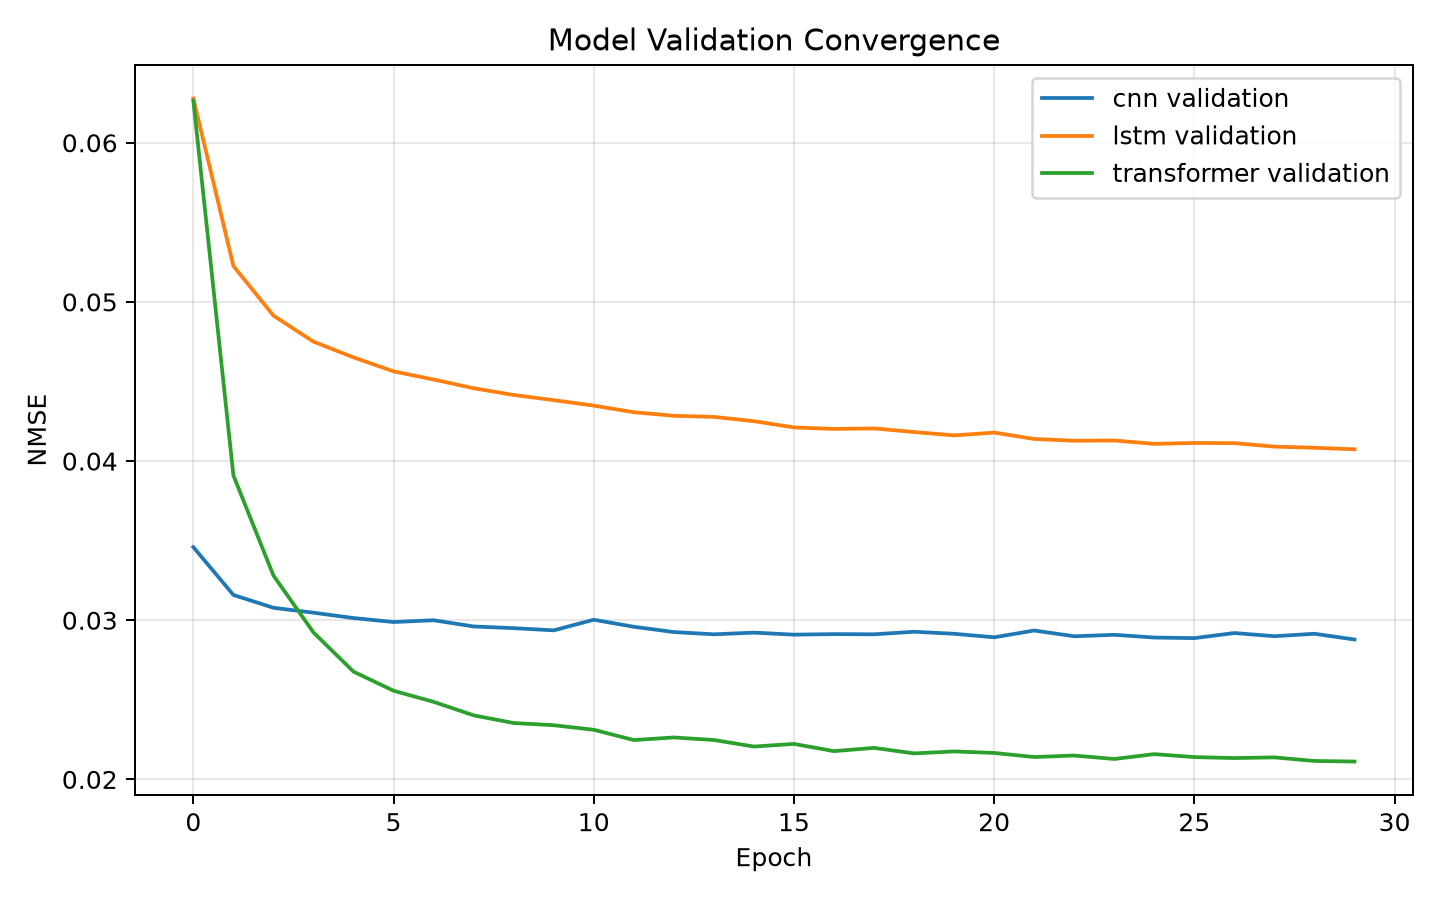
\includegraphics[width=\linewidth]{model_convergence.png}
    \caption{验证集收敛曲线}
  \end{subfigure}
  \caption{三种神经网络的性能与收敛性对比}
  \label{fig:model_compare}
\end{figure}

Transformer 的整体 NMSE 最低，说明全局自注意力能够有效建模跨子载波相关性；其验证 NMSE 在 20 轮内持续下降。LSTM 表现最弱，可能是因为顺序递归对二维天线结构的利用不如卷积直接，同时其参数量约为 CNN 的 7.23 倍。CNN 虽比 Transformer 低约 0.97 dB，但仅有 Transformer 约 7.50\% 的参数量，在资源受限部署中具有更优的精度--规模折中。图~\ref{fig:model_compare}(a) 还显示，CNN 在中高 SNR 多数区间占优，而 Transformer 在低 SNR 下更稳健；不同区间的排序并非完全一致，因此模型选择还应结合目标工作 SNR。

\subsection{信道结构消融实验}

表~\ref{tab:channels} 比较了独立 Rayleigh 与相关多径条件下重新训练后的结果。该组实验与上一节为独立训练运行，模型随机种子也按场景与架构分别设置，因此数值存在正常的训练波动，不能将两个表中的单次运行排名直接混为一谈。

\begin{table}[H]
  \centering
  \caption{不同信道模型下的总体 NMSE（dB）}
  \label{tab:channels}
  \begin{tabular}{llrrr}
    \toprule
    信道 & 模型 & LS & LMMSE & 神经网络 \\
    \midrule
    \multirow{3}{*}{独立 Rayleigh}
      & CNN & $-8.31$ & $-9.97$ & $-9.90$ \\
      & LSTM & $-8.31$ & $-9.97$ & $-9.83$ \\
      & Transformer & $-8.31$ & $-9.97$ & $-9.80$ \\
    \midrule
    \multirow{3}{*}{相关多径}
      & CNN & $-8.27$ & $-9.81$ & $\mathbf{-15.06}$ \\
      & LSTM & $-8.27$ & $-9.81$ & $-12.67$ \\
      & Transformer & $-8.27$ & $-9.81$ & $-14.08$ \\
    \bottomrule
  \end{tabular}
\end{table}

独立 Rayleigh 情形中，各维信道系数之间没有可供网络利用的相关性，三种网络均接近但略差于 LMMSE，差距为 0.07--0.17 dB。该结果说明实验没有表现出不合理的“无结构增益”，也从侧面支持训练与测试数据相互独立。相关多径情形下，CNN、LSTM、Transformer 分别比 LMMSE 改善 5.25、2.86 和 4.27 dB；其中 CNN 在该次独立运行中取得最佳结果。由此可见，神经估计器的主要增益来源不是简单记忆，而是对空间相关性、有限多径和频域平滑性的联合利用。

\subsection{统一架构实验的信道重构与残差诊断}

图~\ref{fig:model_heatmaps} 汇总了架构对比实验中三种网络在接近 10 dB 的同类样本上的诊断结果。每张图同时展示真实信道、LS、LMMSE 和网络输出，且使用统一色标，因而可以直接判断网络是否在降噪时破坏了空间幅度结构。

\begin{figure}[H]
  \centering
  \begin{subfigure}[t]{0.58\textwidth}
    \centering
    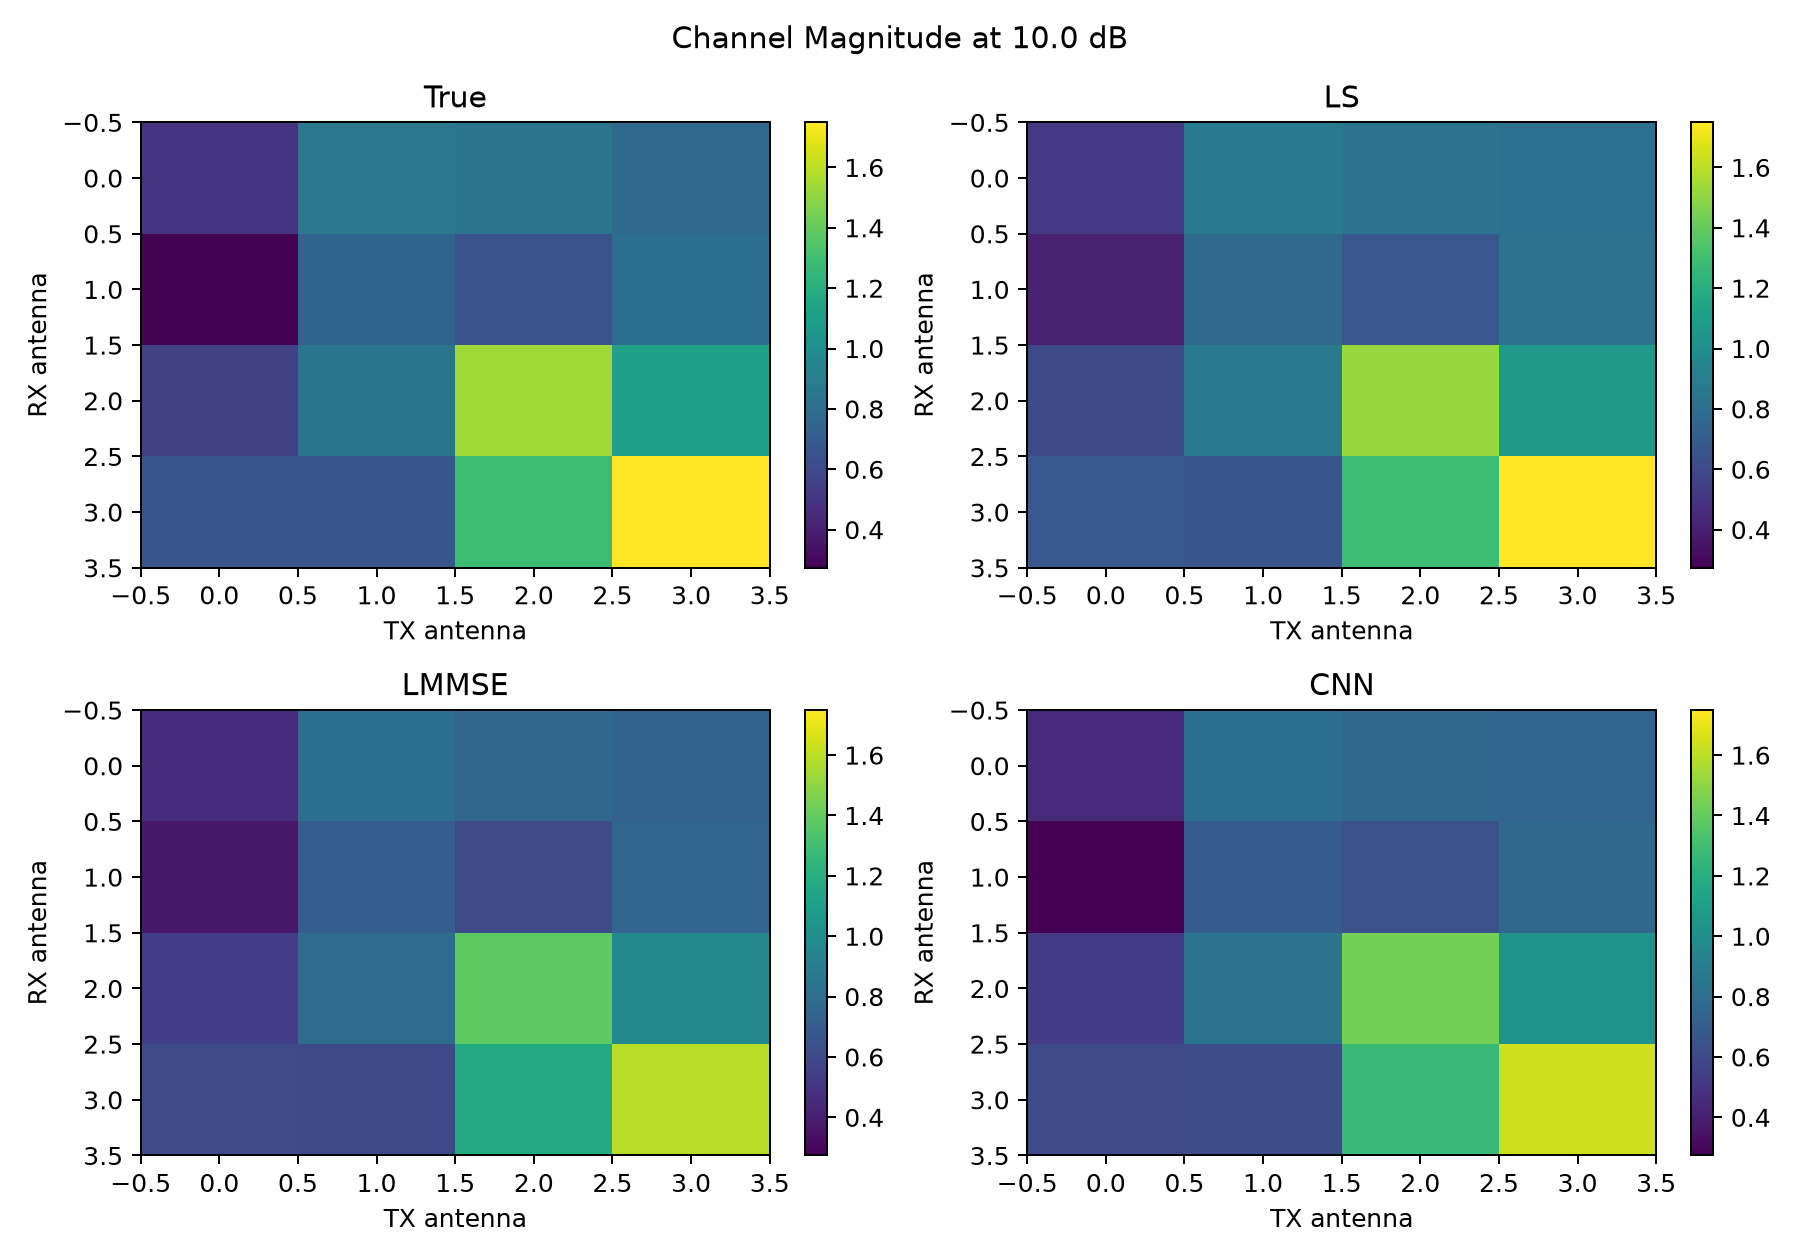
\includegraphics[width=\linewidth]{models/cnn_heatmap.png}
    \caption{CNN：局部平滑明显，主要强弱区域得到保持}
  \end{subfigure}

  \begin{subfigure}[t]{0.58\textwidth}
    \centering
    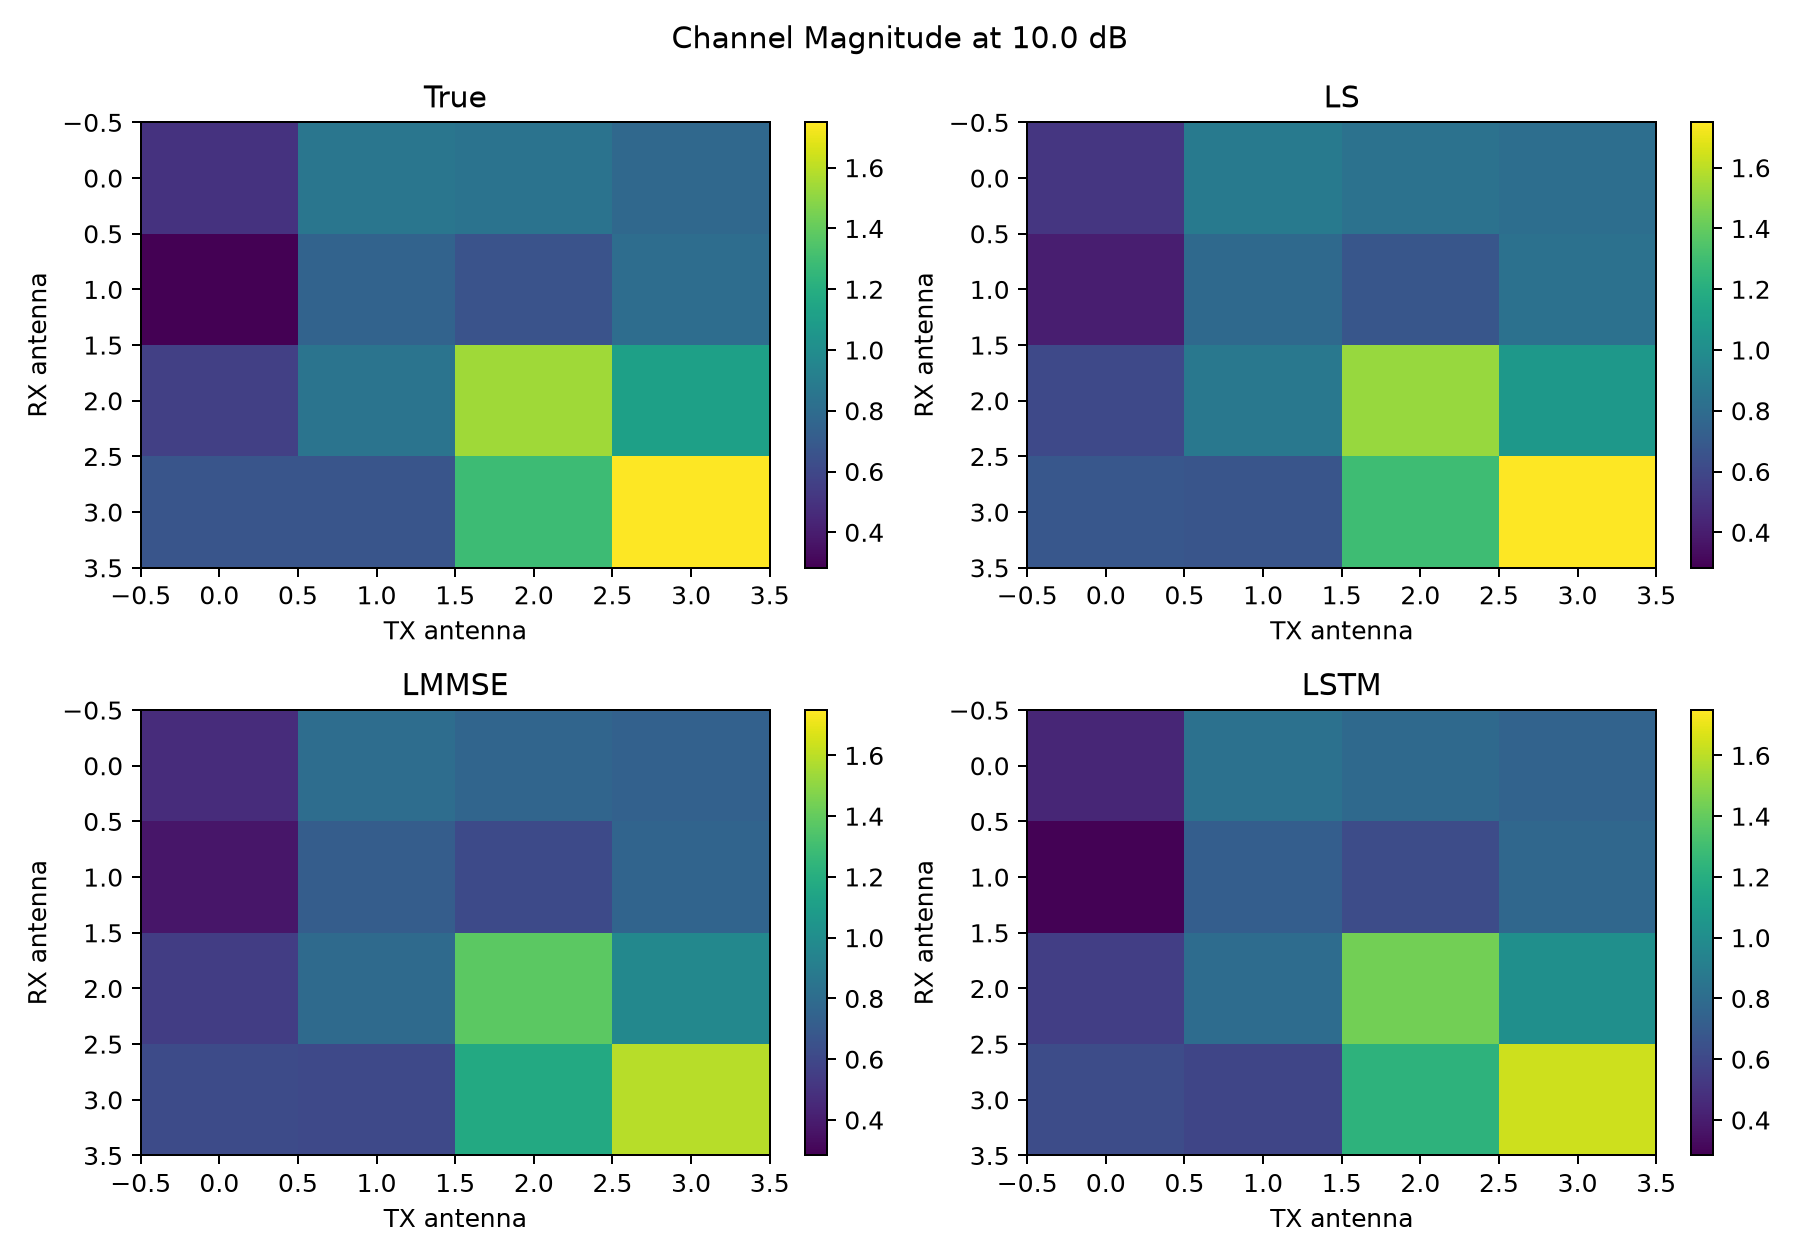
\includegraphics[width=\linewidth]{models/lstm_heatmap.png}
    \caption{LSTM：总体空间轮廓正确，但局部幅度偏差相对更明显}
  \end{subfigure}

  \begin{subfigure}[t]{0.58\textwidth}
    \centering
    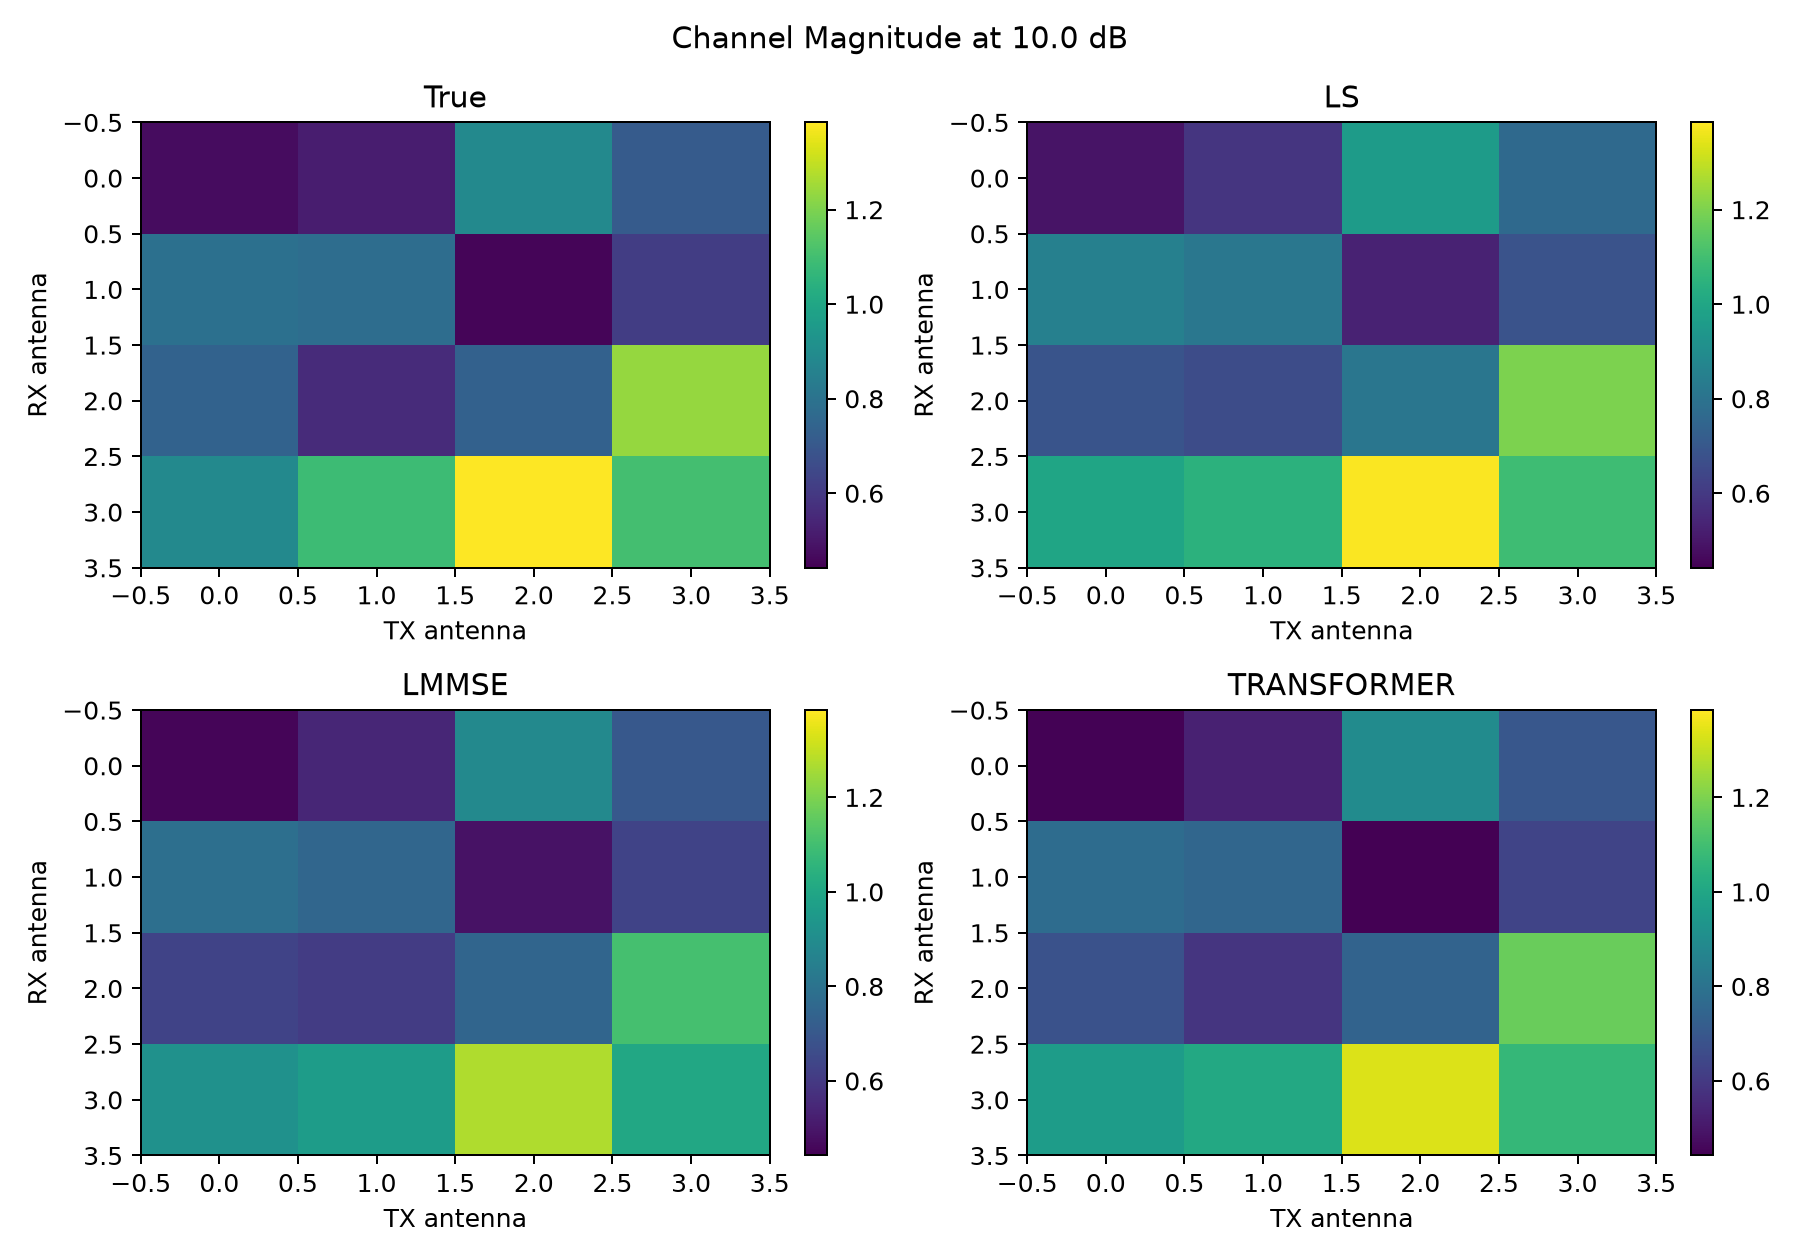
\includegraphics[width=\linewidth]{models/transformer_heatmap.png}
    \caption{Transformer：对整体结构与跨位置关系的恢复较充分}
  \end{subfigure}
  \caption{CNN、LSTM、Transformer 的统一四联信道幅度诊断图}
  \label{fig:model_heatmaps}
\end{figure}

图~\ref{fig:model_residuals} 给出了同一架构实验中的完整残差对比。三张图都以 LS、LMMSE 和网络预测误差为对象，网络曲线越高且越窄地集中在零附近，代表多数实部/虚部分量的误差越小。CNN 与 Transformer 的中心峰更集中，与二者更低的总体 NMSE 相符；LSTM 也明显压缩了传统基线的残差，但尾部更宽，对应其总体精度略低。三类网络均存在长尾，说明低 SNR 或少量困难样本仍会造成较大的分量误差。

\begin{figure}[H]
  \centering
  \begin{subfigure}[t]{0.32\textwidth}
    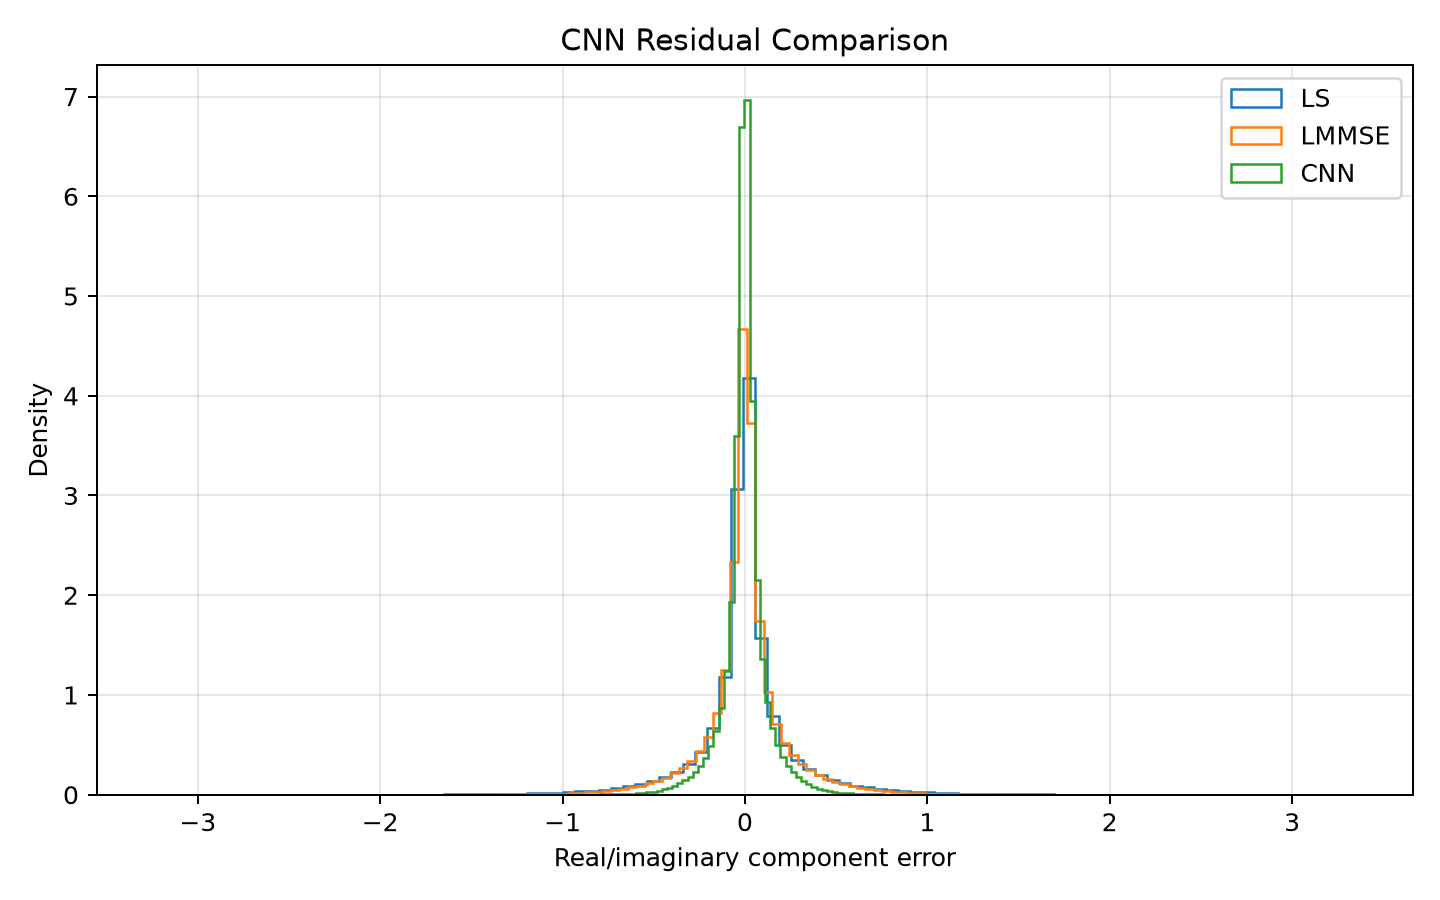
\includegraphics[width=\linewidth]{models/cnn_residual.png}
    \caption{CNN}
  \end{subfigure}\hfill
  \begin{subfigure}[t]{0.32\textwidth}
    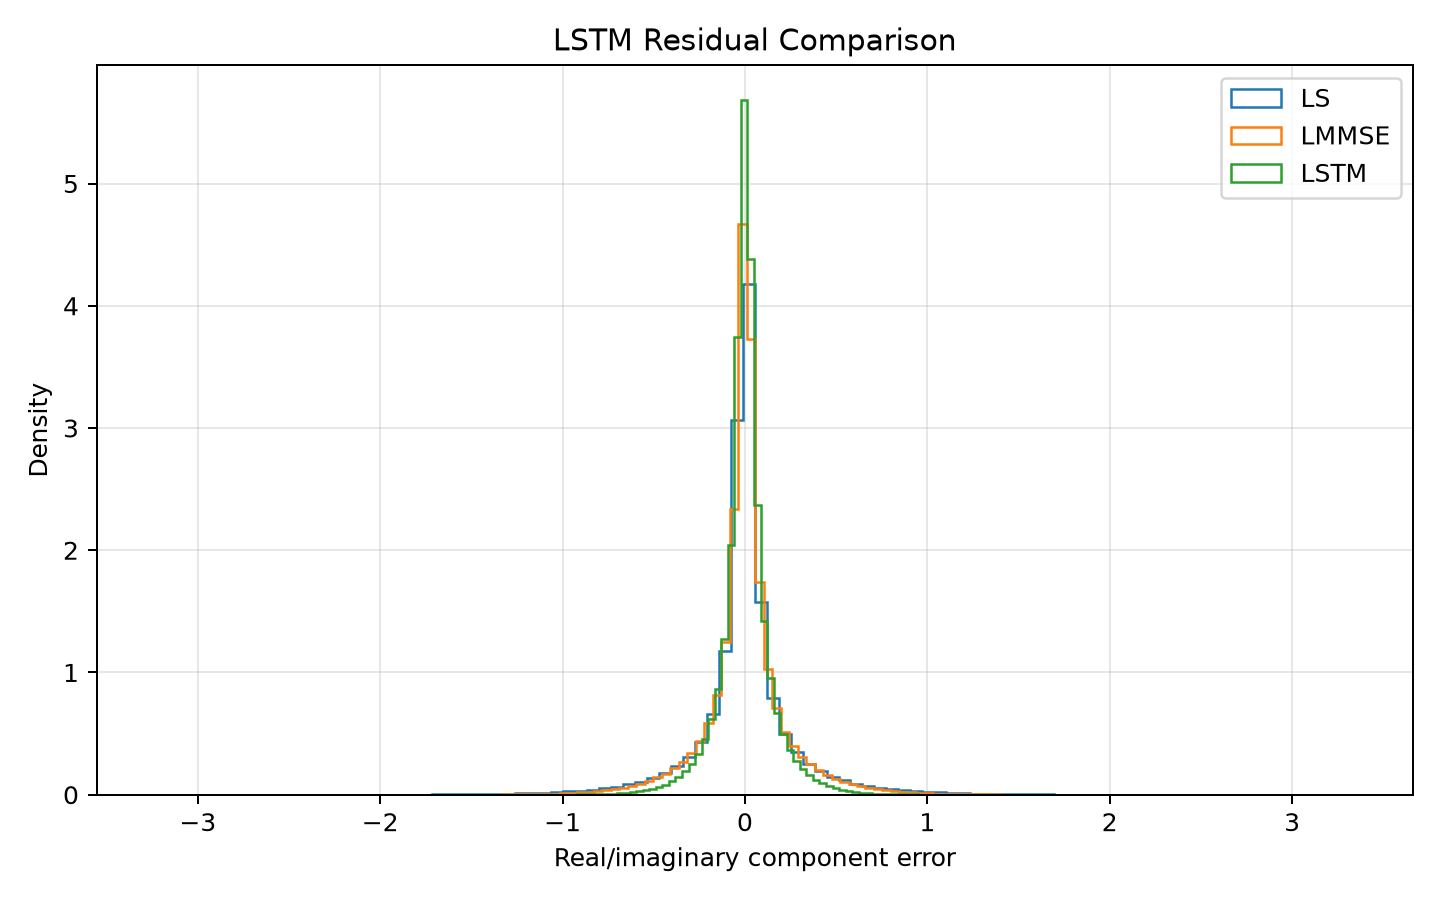
\includegraphics[width=\linewidth]{models/lstm_residual.png}
    \caption{LSTM}
  \end{subfigure}\hfill
  \begin{subfigure}[t]{0.32\textwidth}
    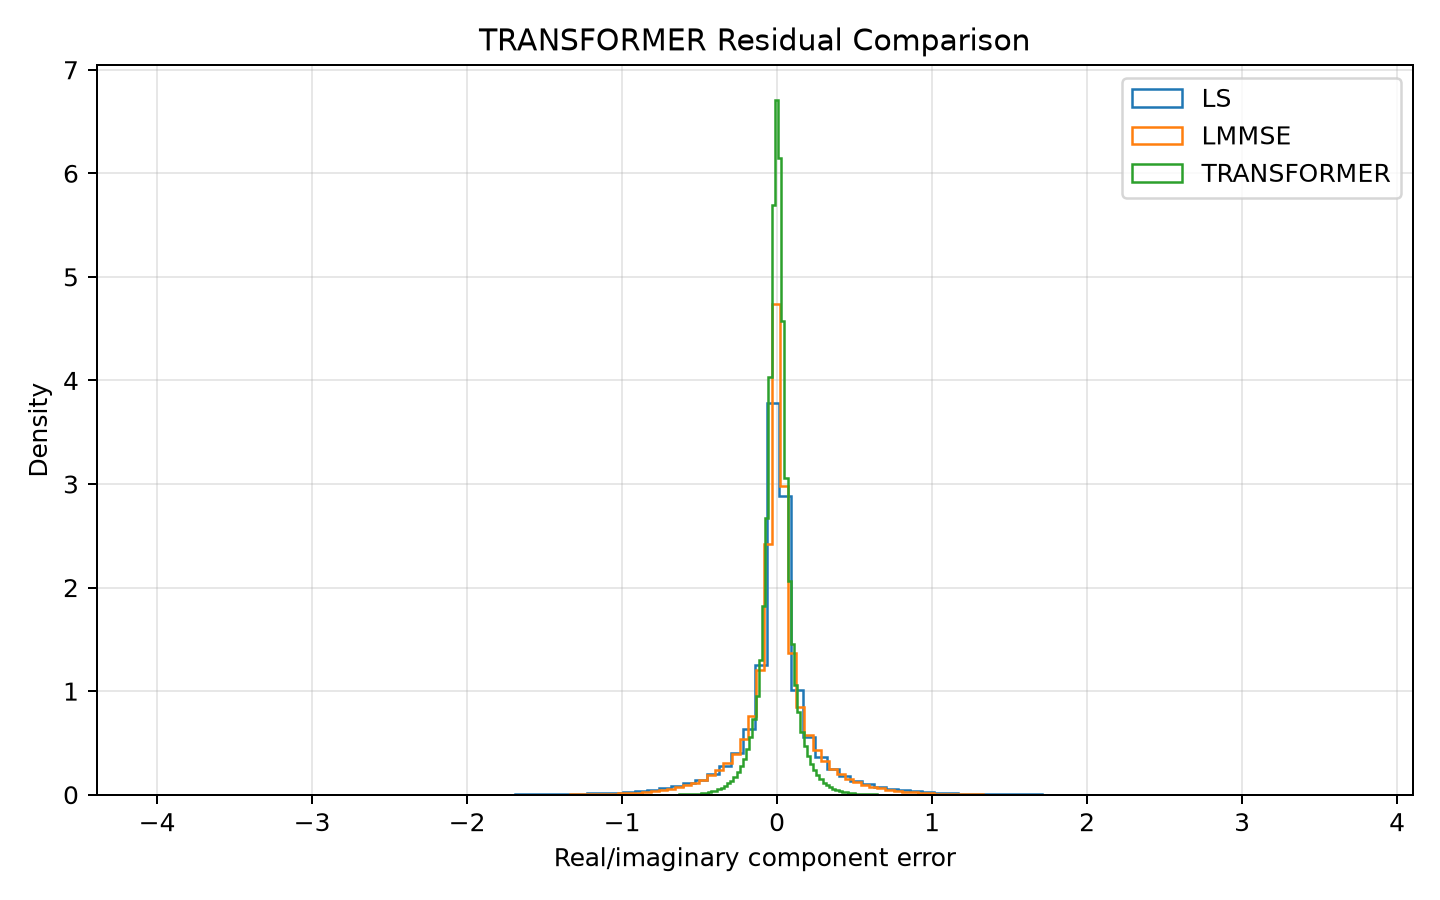
\includegraphics[width=\linewidth]{models/transformer_residual.png}
    \caption{Transformer}
  \end{subfigure}
  \caption{三种架构与 LS、LMMSE 的残差概率密度对比}
  \label{fig:model_residuals}
\end{figure}

\subsection{独立 Rayleigh 信道的完整图像矩阵}

图~\ref{fig:rayleigh_loss} 显示，三种网络的训练和验证 NMSE 均在前几轮快速下降，随后逐渐逼近标量 LMMSE 水平。CNN 的验证曲线在约第 6 轮后已贴近基线；LSTM 与 Transformer 虽持续下降，但 12 轮结束时仍没有形成稳定的基线优势。这与表~\ref{tab:channels} 中三种网络均略逊于 LMMSE 的测试结果一致，而不是由某一张样本图偶然造成。

\begin{figure}[H]
  \centering
  \begin{subfigure}[t]{0.32\textwidth}
    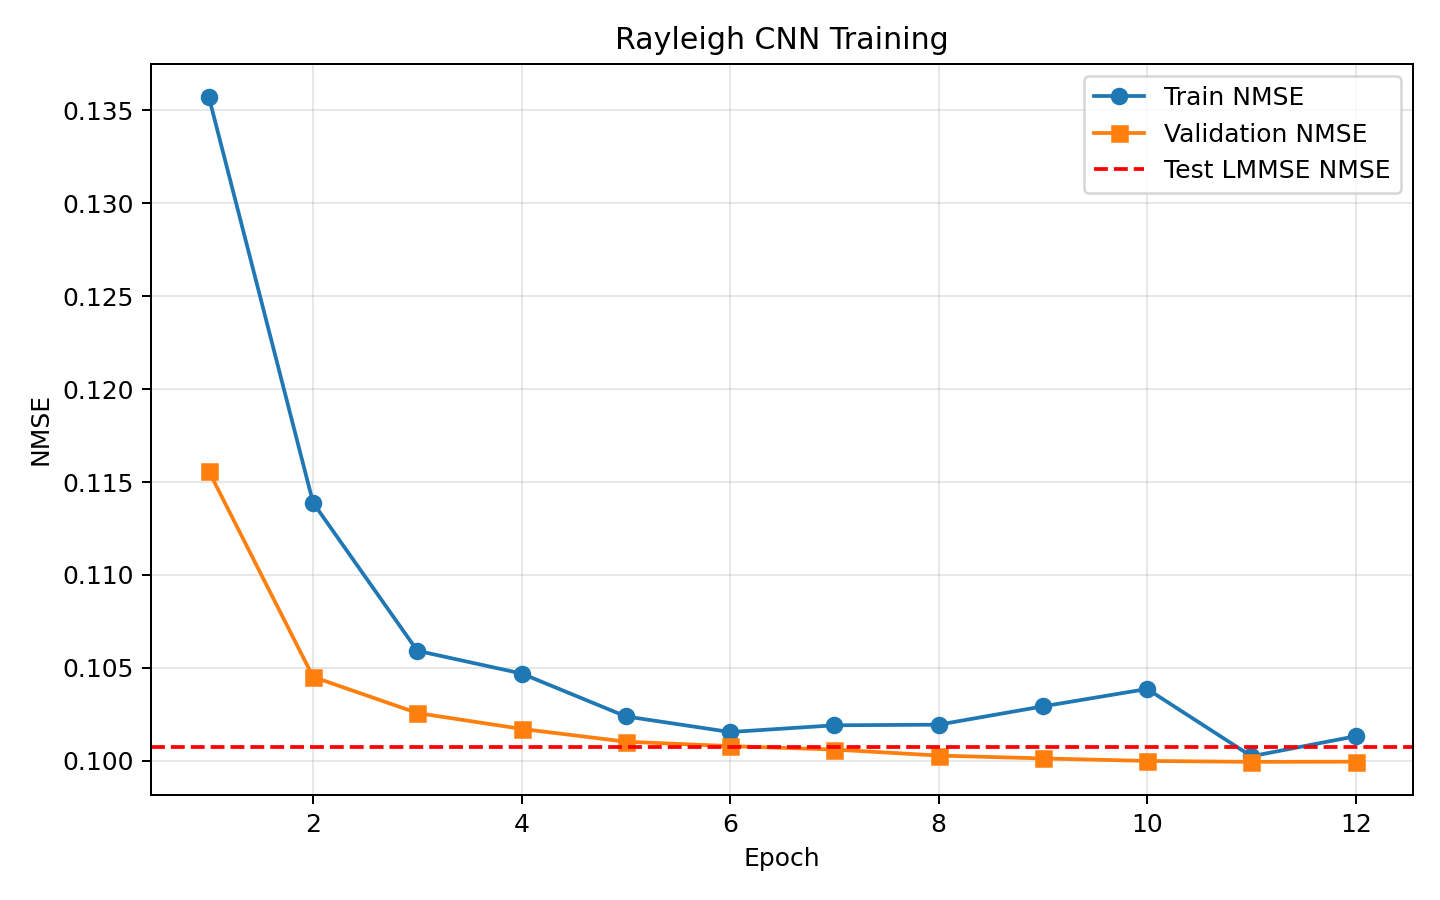
\includegraphics[width=\linewidth]{Rayleigh_cnn_LossCurve.png}
    \caption{CNN}
  \end{subfigure}\hfill
  \begin{subfigure}[t]{0.32\textwidth}
    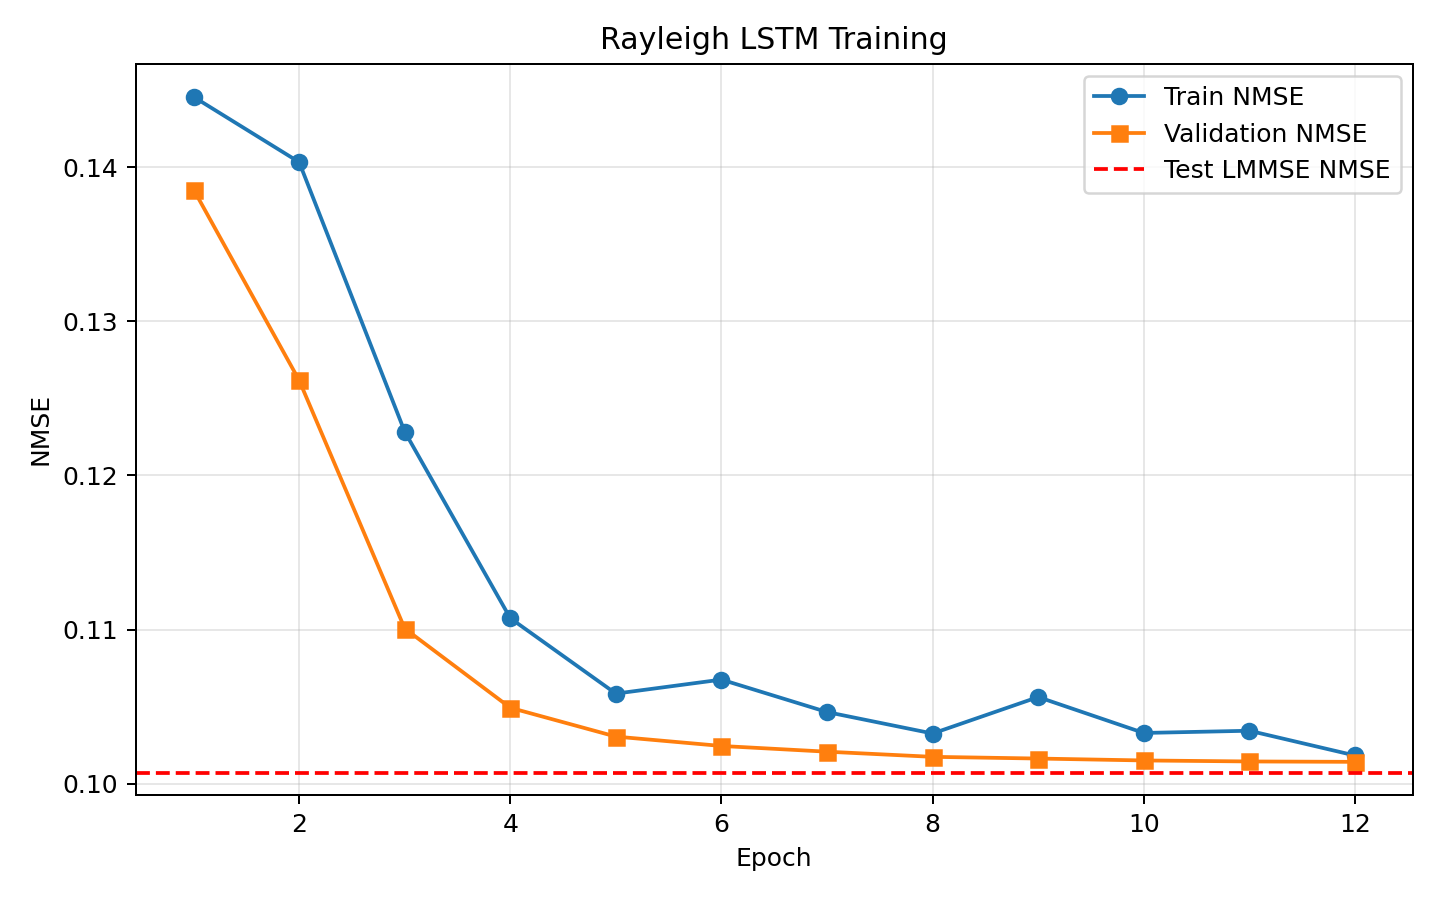
\includegraphics[width=\linewidth]{Rayleigh_lstm_LossCurve.png}
    \caption{LSTM}
  \end{subfigure}\hfill
  \begin{subfigure}[t]{0.32\textwidth}
    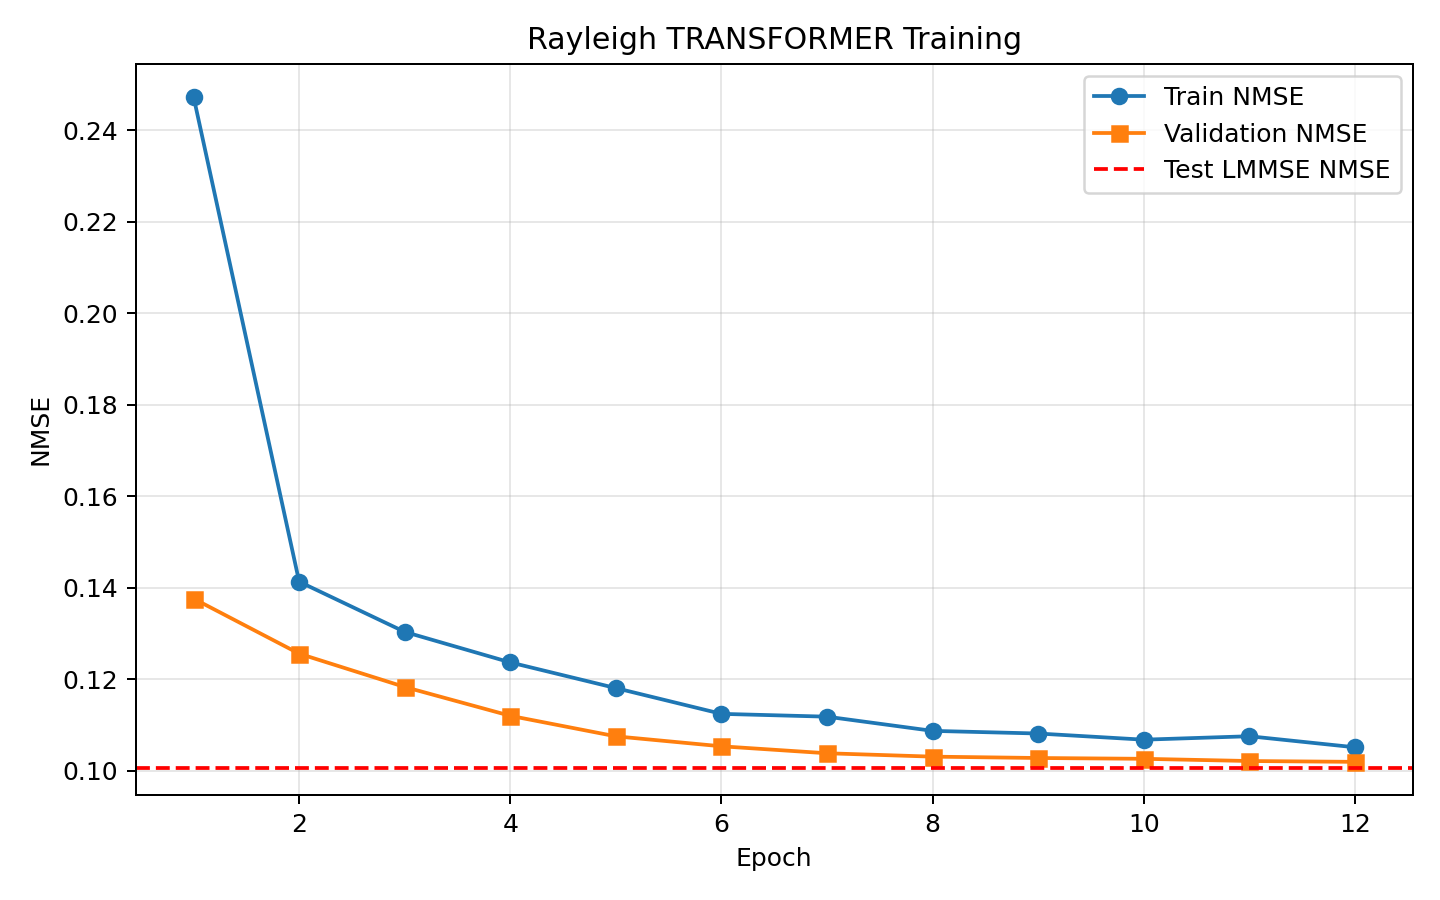
\includegraphics[width=\linewidth]{Rayleigh_transformer_LossCurve.png}
    \caption{Transformer}
  \end{subfigure}
  \caption{独立 Rayleigh 信道下的训练与验证 NMSE 曲线；红色虚线为测试集 LMMSE NMSE}
  \label{fig:rayleigh_loss}
\end{figure}

图~\ref{fig:rayleigh_heat} 中，三个模型都能大致恢复所选样本的 $4\times4$ 空间幅度分布，但局部单元仍存在可见的增强或衰减偏差。由于独立 Rayleigh 系数在空间和频率上没有稳定邻域关系，网络无法像在多径场景中那样利用相邻位置完成可靠去噪；单样本视觉上“相似”并不等价于总体统计性能超过 LMMSE。

\begin{figure}[H]
  \centering
  \begin{subfigure}[t]{0.32\textwidth}
    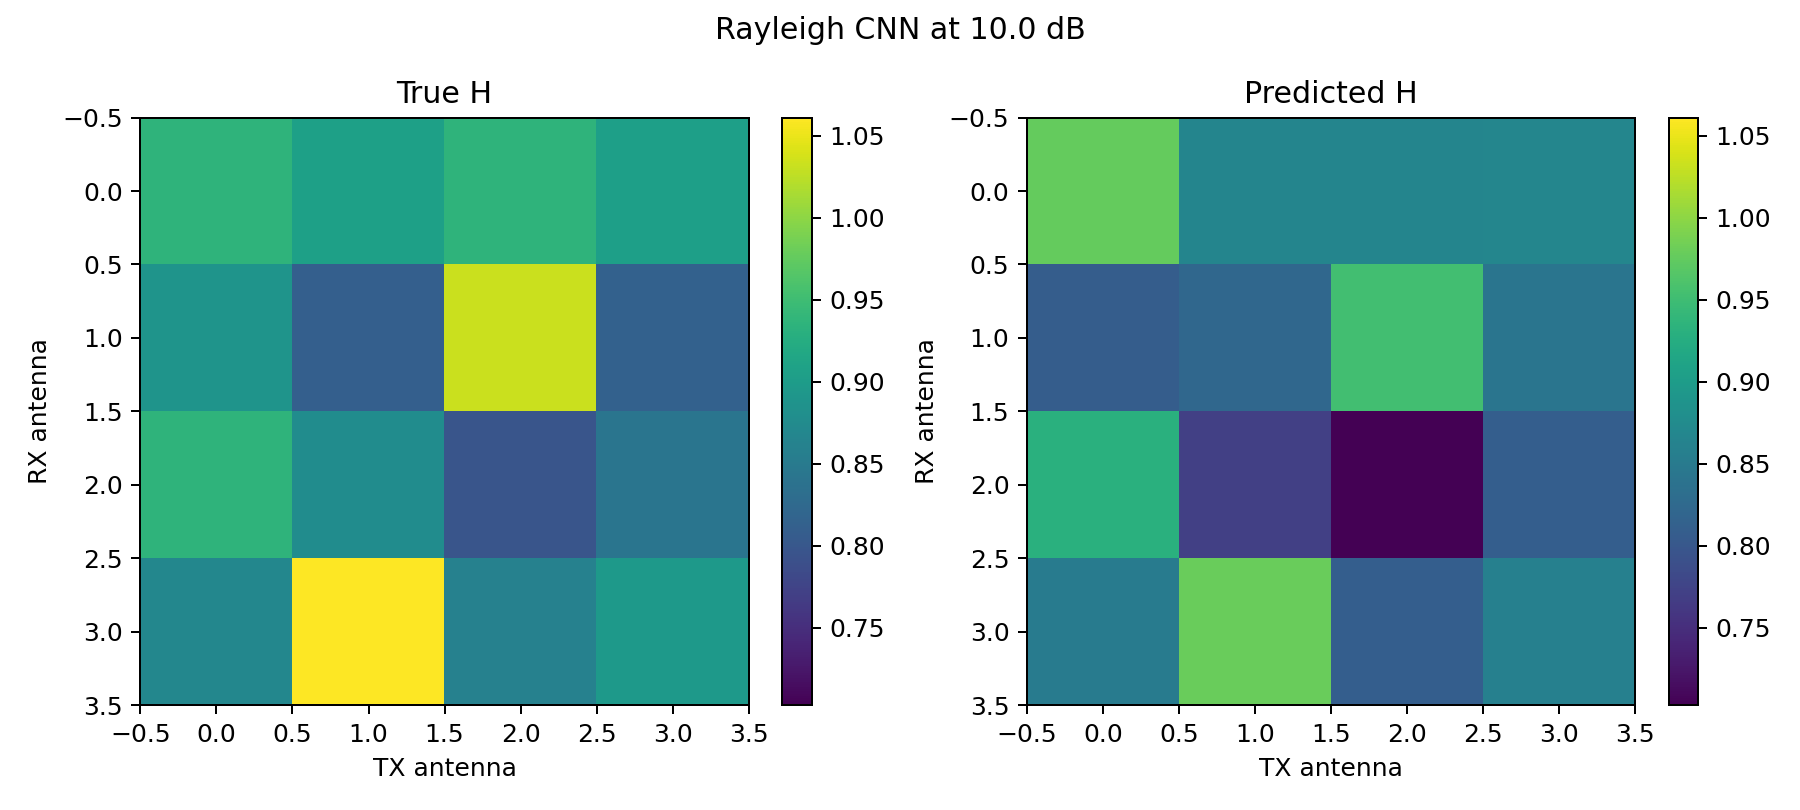
\includegraphics[width=\linewidth]{Rayleigh_cnn_Heatmap.png}
    \caption{CNN}
  \end{subfigure}\hfill
  \begin{subfigure}[t]{0.32\textwidth}
    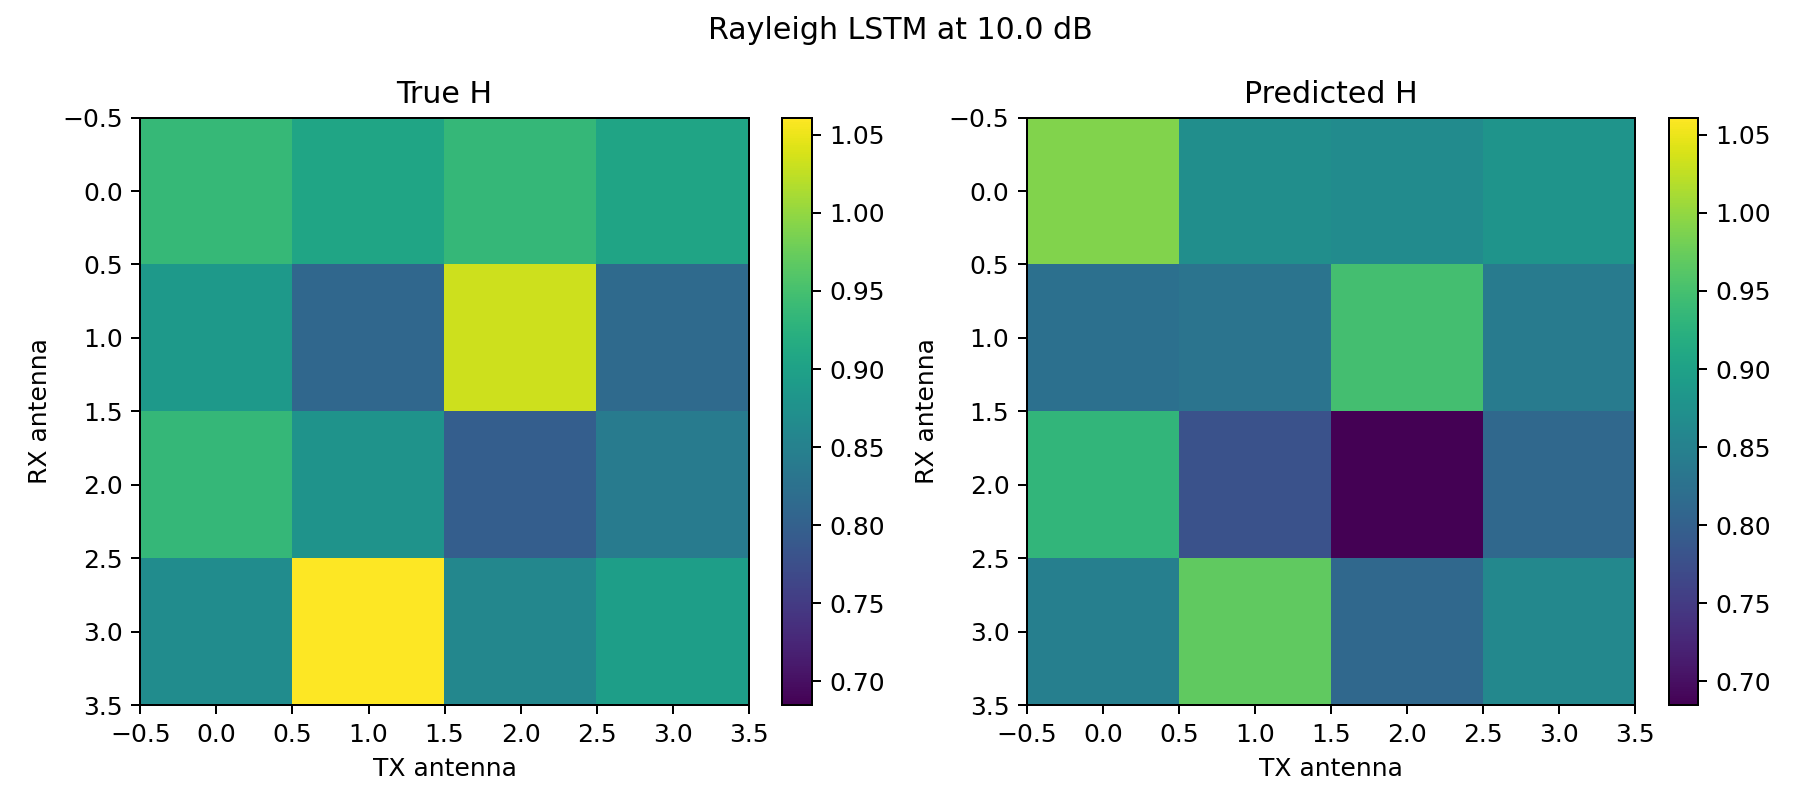
\includegraphics[width=\linewidth]{Rayleigh_lstm_Heatmap.png}
    \caption{LSTM}
  \end{subfigure}\hfill
  \begin{subfigure}[t]{0.32\textwidth}
    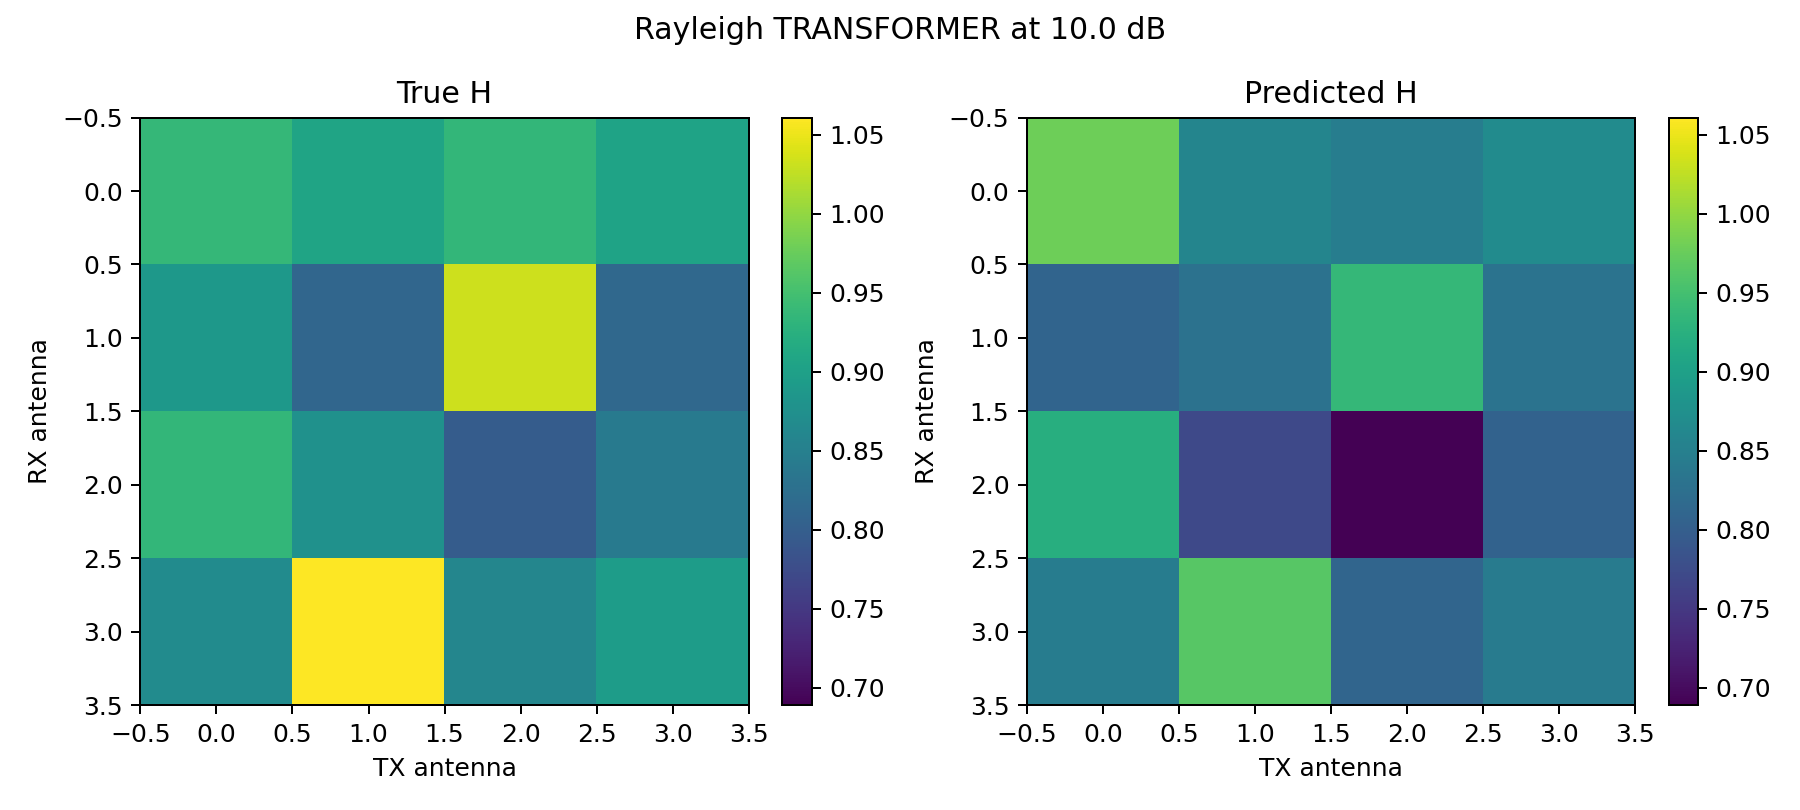
\includegraphics[width=\linewidth]{Rayleigh_transformer_Heatmap.png}
    \caption{Transformer}
  \end{subfigure}
  \caption{独立 Rayleigh 信道在约 10 dB 时的真实幅度与预测幅度}
  \label{fig:rayleigh_heat}
\end{figure}

图~\ref{fig:rayleigh_residual} 中三类模型的残差均以零为中心且形状近似对称，说明没有显著的系统性正负偏置；但分布仍具有较宽尾部。结合约 $-9.8$ 至 $-9.9$ dB 的总体 NMSE，可判断此时网络主要学到了接近标量收缩的映射，复杂架构并未凭空创造独立信道中不存在的相关信息。

\begin{figure}[H]
  \centering
  \begin{subfigure}[t]{0.32\textwidth}
    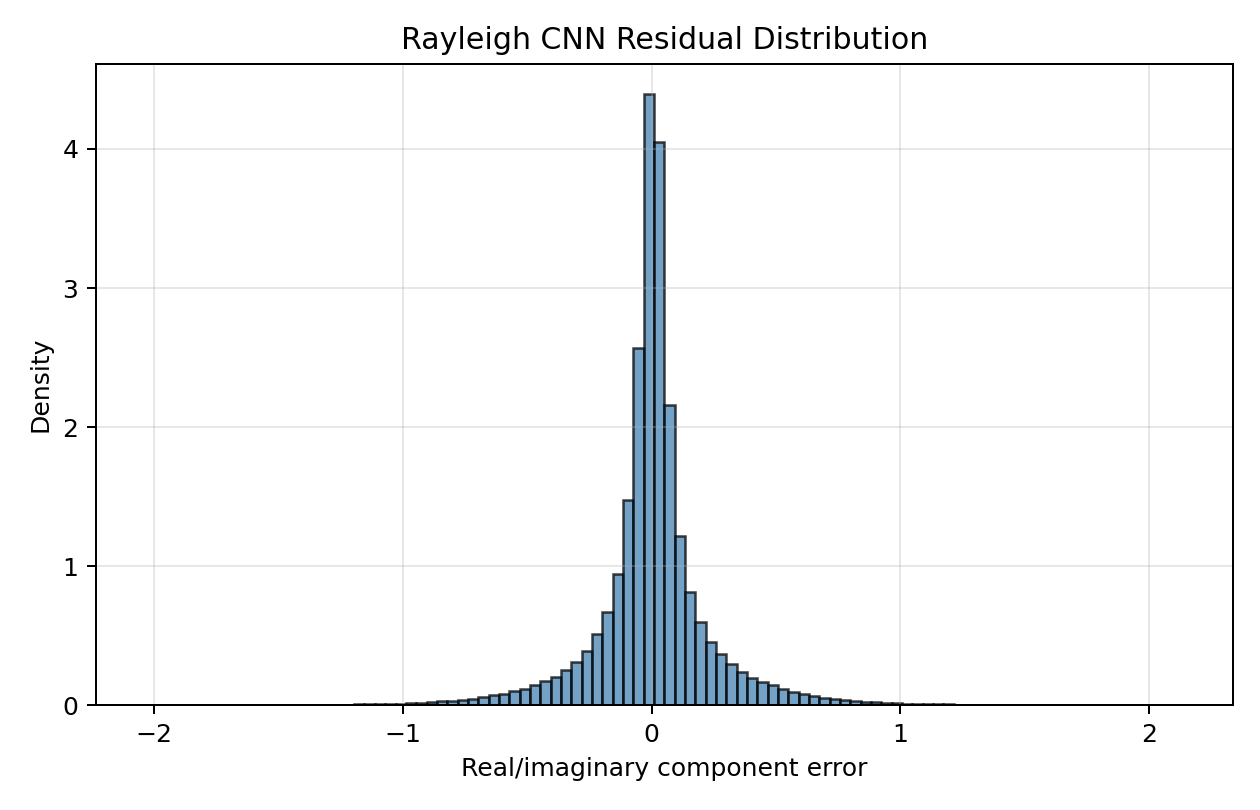
\includegraphics[width=\linewidth]{Rayleigh_cnn_ResidualHistogram.png}
    \caption{CNN}
  \end{subfigure}\hfill
  \begin{subfigure}[t]{0.32\textwidth}
    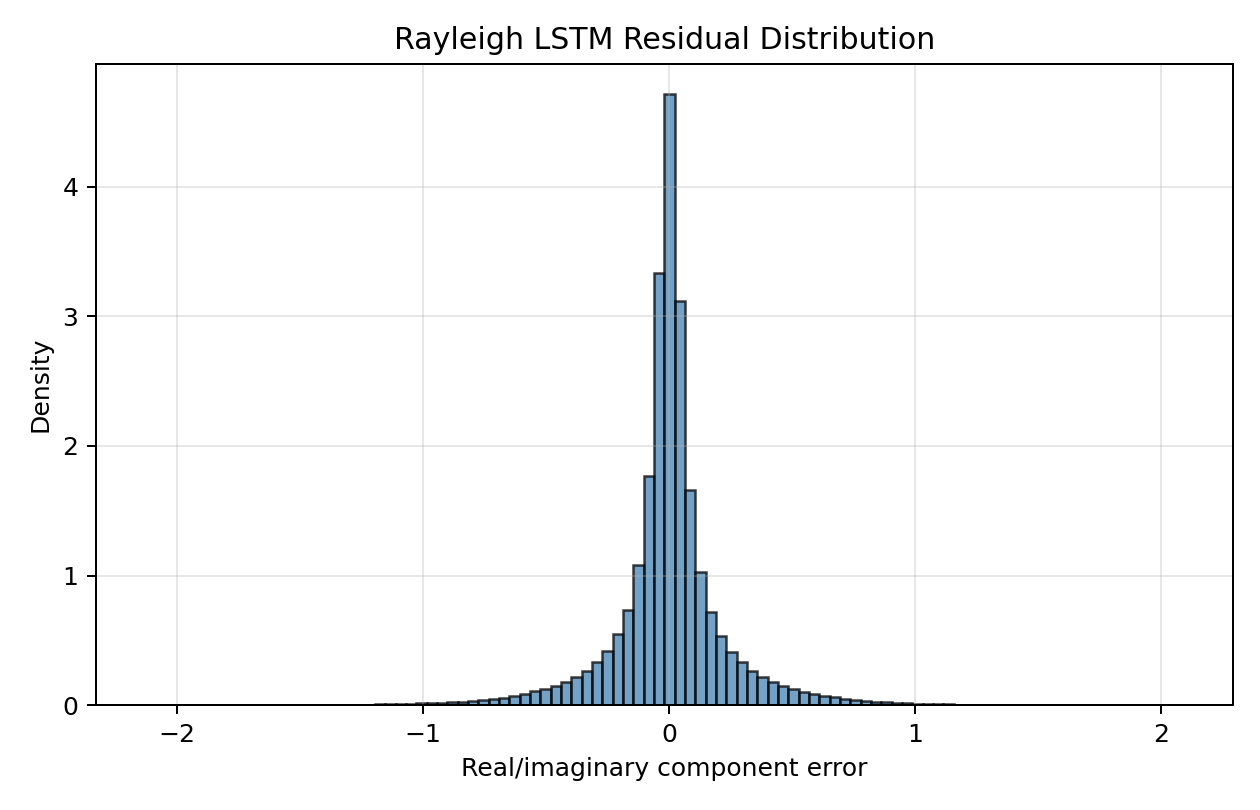
\includegraphics[width=\linewidth]{Rayleigh_lstm_ResidualHistogram.png}
    \caption{LSTM}
  \end{subfigure}\hfill
  \begin{subfigure}[t]{0.32\textwidth}
    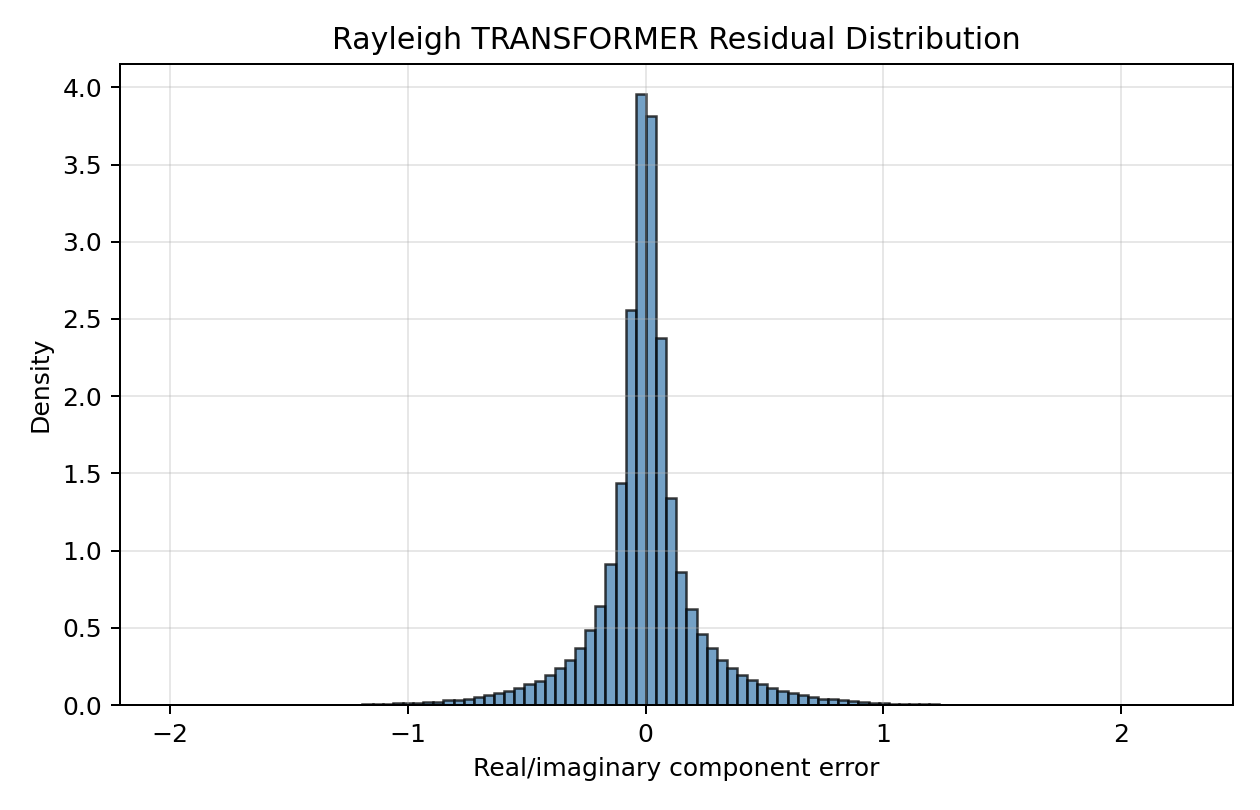
\includegraphics[width=\linewidth]{Rayleigh_transformer_ResidualHistogram.png}
    \caption{Transformer}
  \end{subfigure}
  \caption{独立 Rayleigh 信道下三种网络的实部/虚部残差分布}
  \label{fig:rayleigh_residual}
\end{figure}

\subsection{相关多径信道的完整图像矩阵}

多径场景的训练曲线见图~\ref{fig:multipath_loss}。CNN 在第二轮便明显越过 LMMSE 基线，之后快速收敛至约 0.026 的验证 NMSE；Transformer 在第二轮附近越过基线并持续改善；LSTM 收敛较慢，但从第四轮开始也稳定优于基线。训练与验证曲线走势一致，未出现明显的后期发散，其中 CNN 的收敛速度和最终水平在该次场景实验中最好。

\begin{figure}[H]
  \centering
  \begin{subfigure}[t]{0.32\textwidth}
    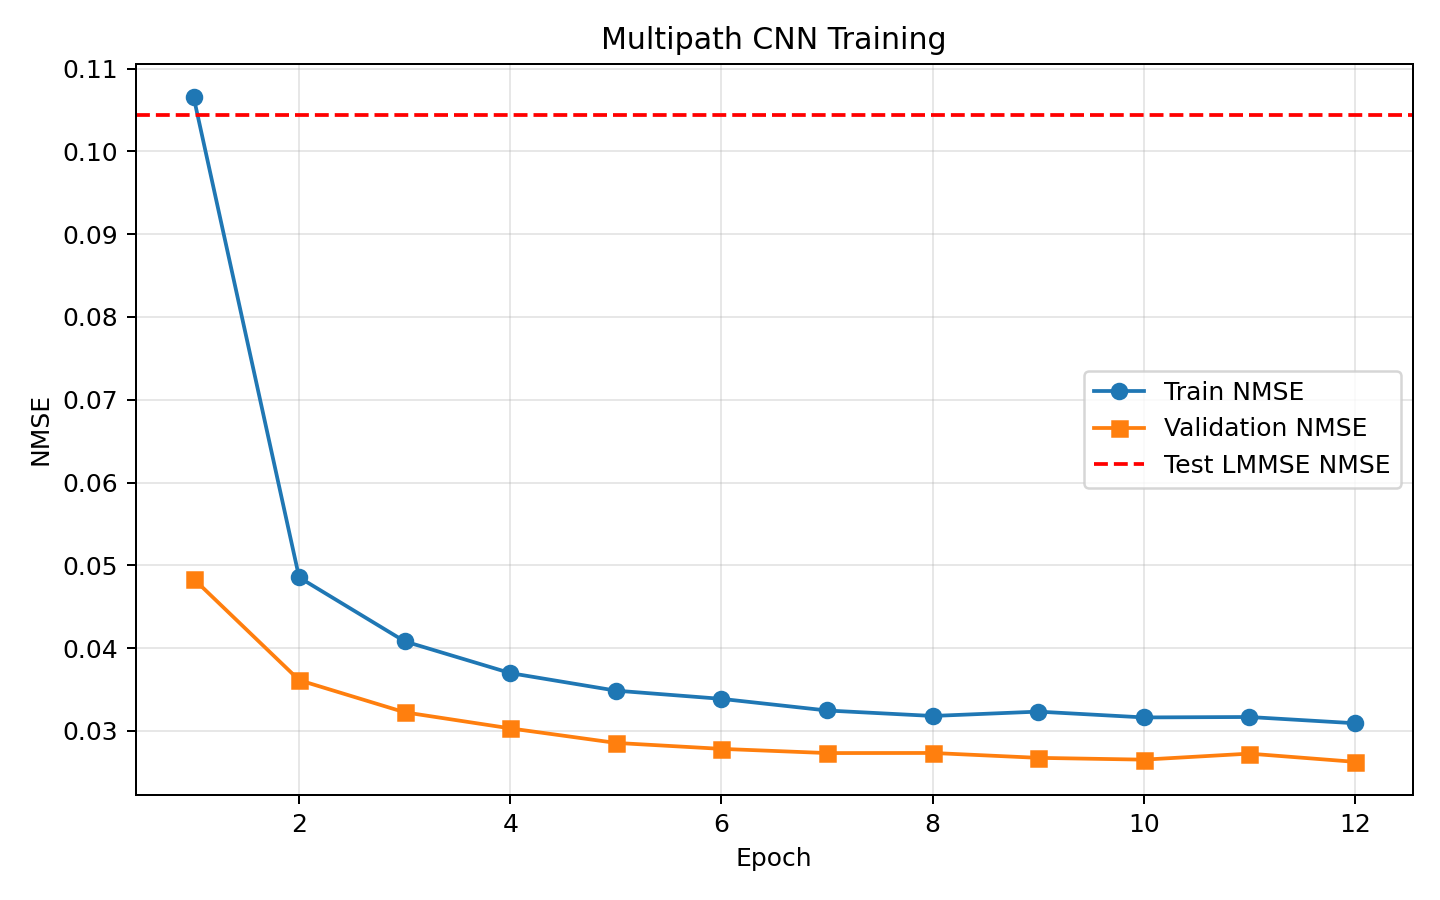
\includegraphics[width=\linewidth]{Multipath_cnn_LossCurve.png}
    \caption{CNN}
  \end{subfigure}\hfill
  \begin{subfigure}[t]{0.32\textwidth}
    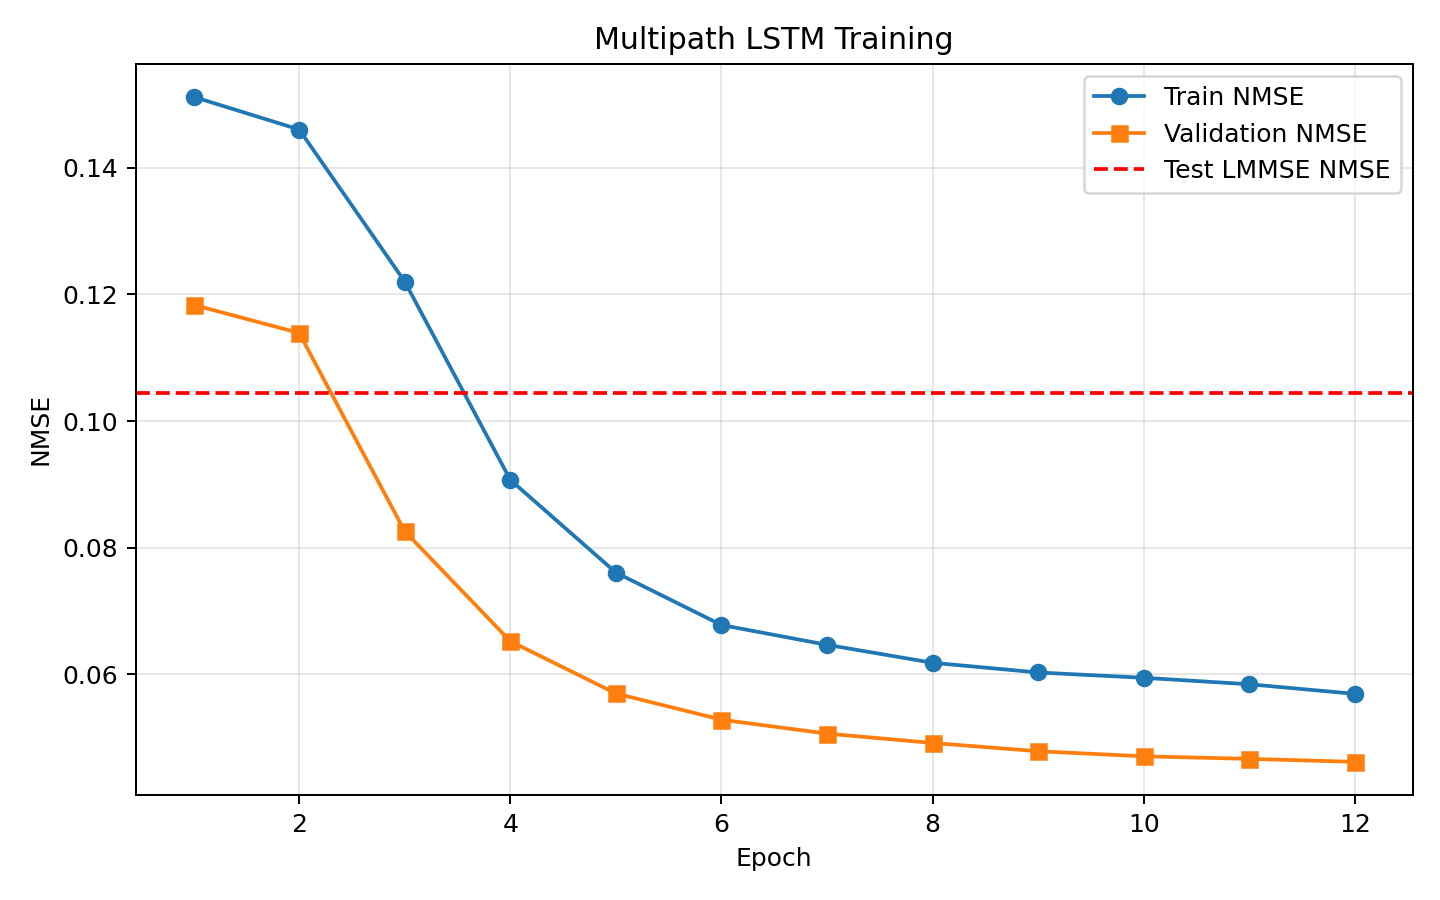
\includegraphics[width=\linewidth]{Multipath_lstm_LossCurve.png}
    \caption{LSTM}
  \end{subfigure}\hfill
  \begin{subfigure}[t]{0.32\textwidth}
    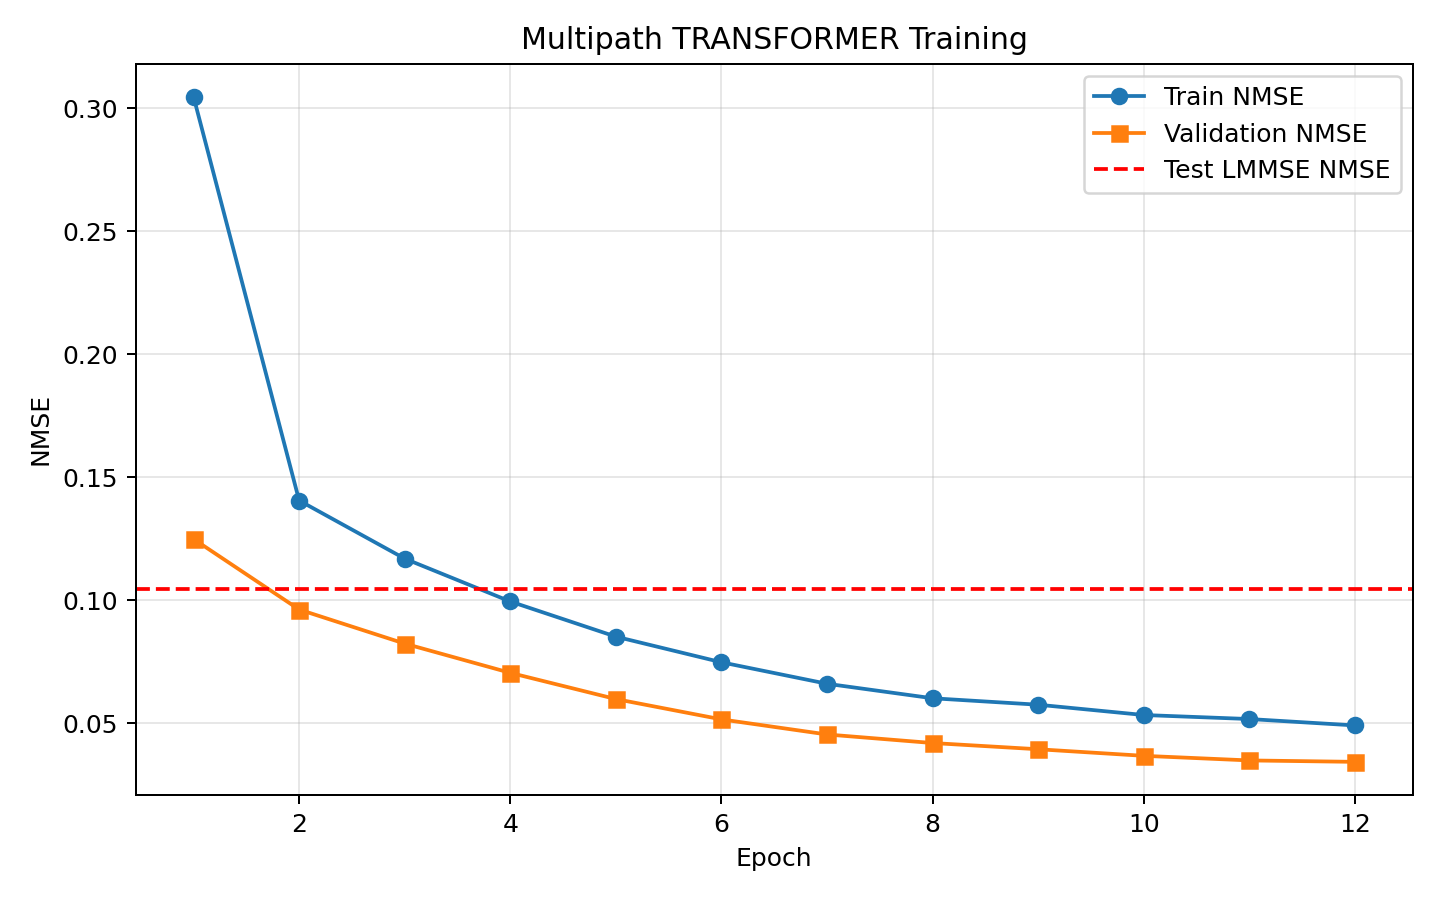
\includegraphics[width=\linewidth]{Multipath_transformer_LossCurve.png}
    \caption{Transformer}
  \end{subfigure}
  \caption{相关多径信道下的训练与验证 NMSE 曲线；红色虚线为测试集 LMMSE NMSE}
  \label{fig:multipath_loss}
\end{figure}

图~\ref{fig:multipath_heat} 展示了三个模型各自测试集中接近 10 dB 的样本。三者均能保持真实信道的主要空间强弱格局；CNN 和 Transformer 对相邻天线间平滑结构的恢复尤其清晰，LSTM 也能恢复整体模式但局部幅度偏差更大。这一视觉差异与场景实验中 CNN、Transformer 优于 LSTM 的定量排序一致。

\begin{figure}[H]
  \centering
  \begin{subfigure}[t]{0.32\textwidth}
    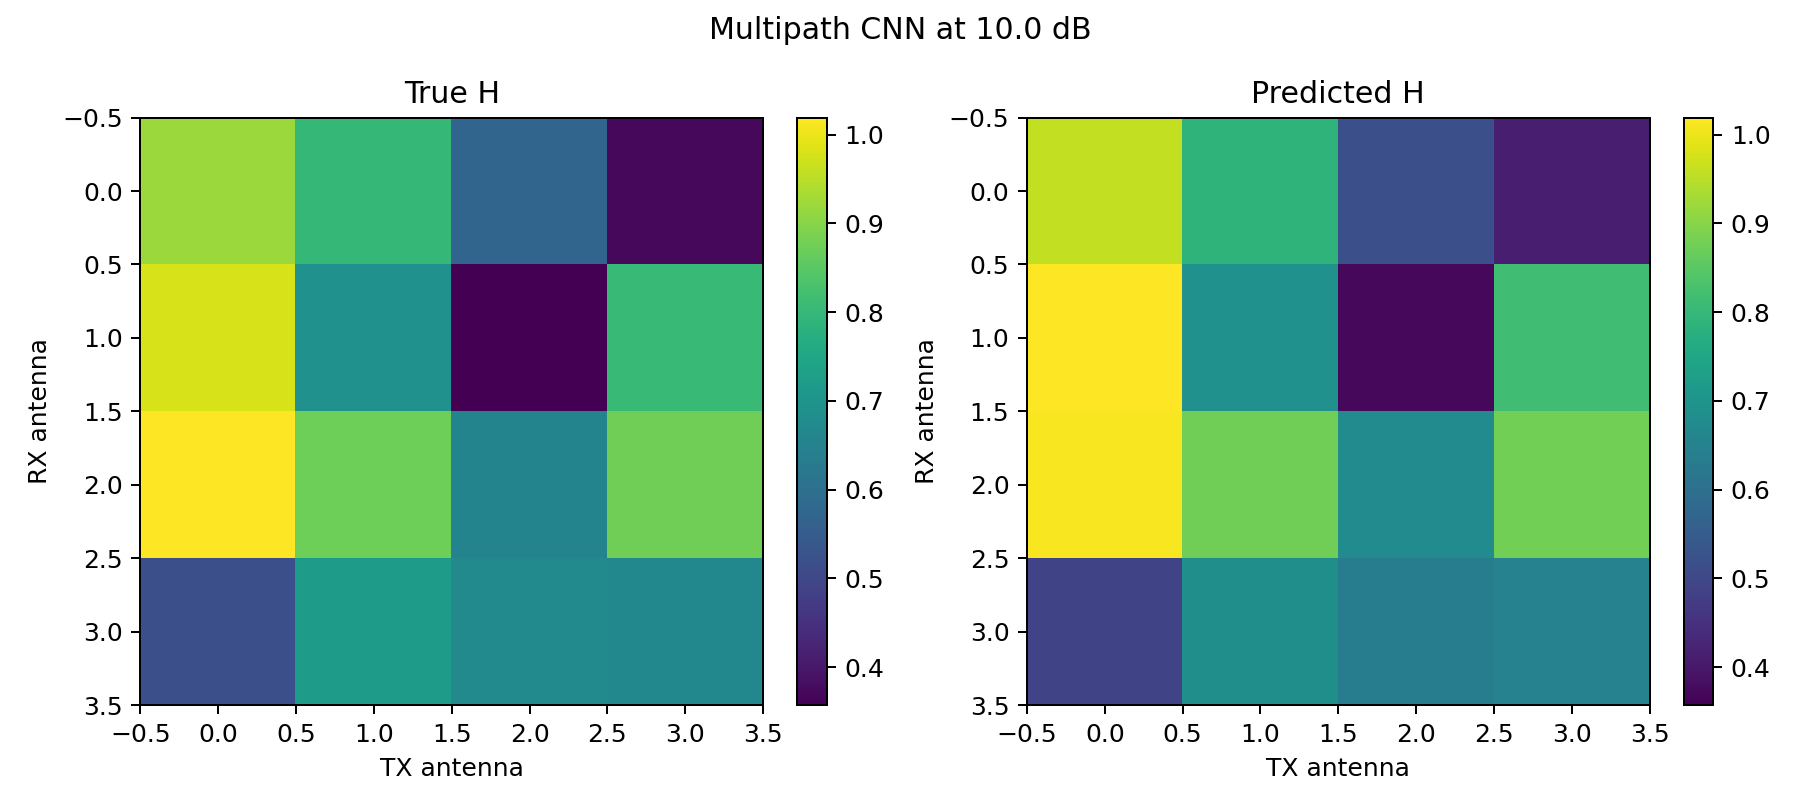
\includegraphics[width=\linewidth]{Multipath_cnn_Heatmap.png}
    \caption{CNN}
  \end{subfigure}\hfill
  \begin{subfigure}[t]{0.32\textwidth}
    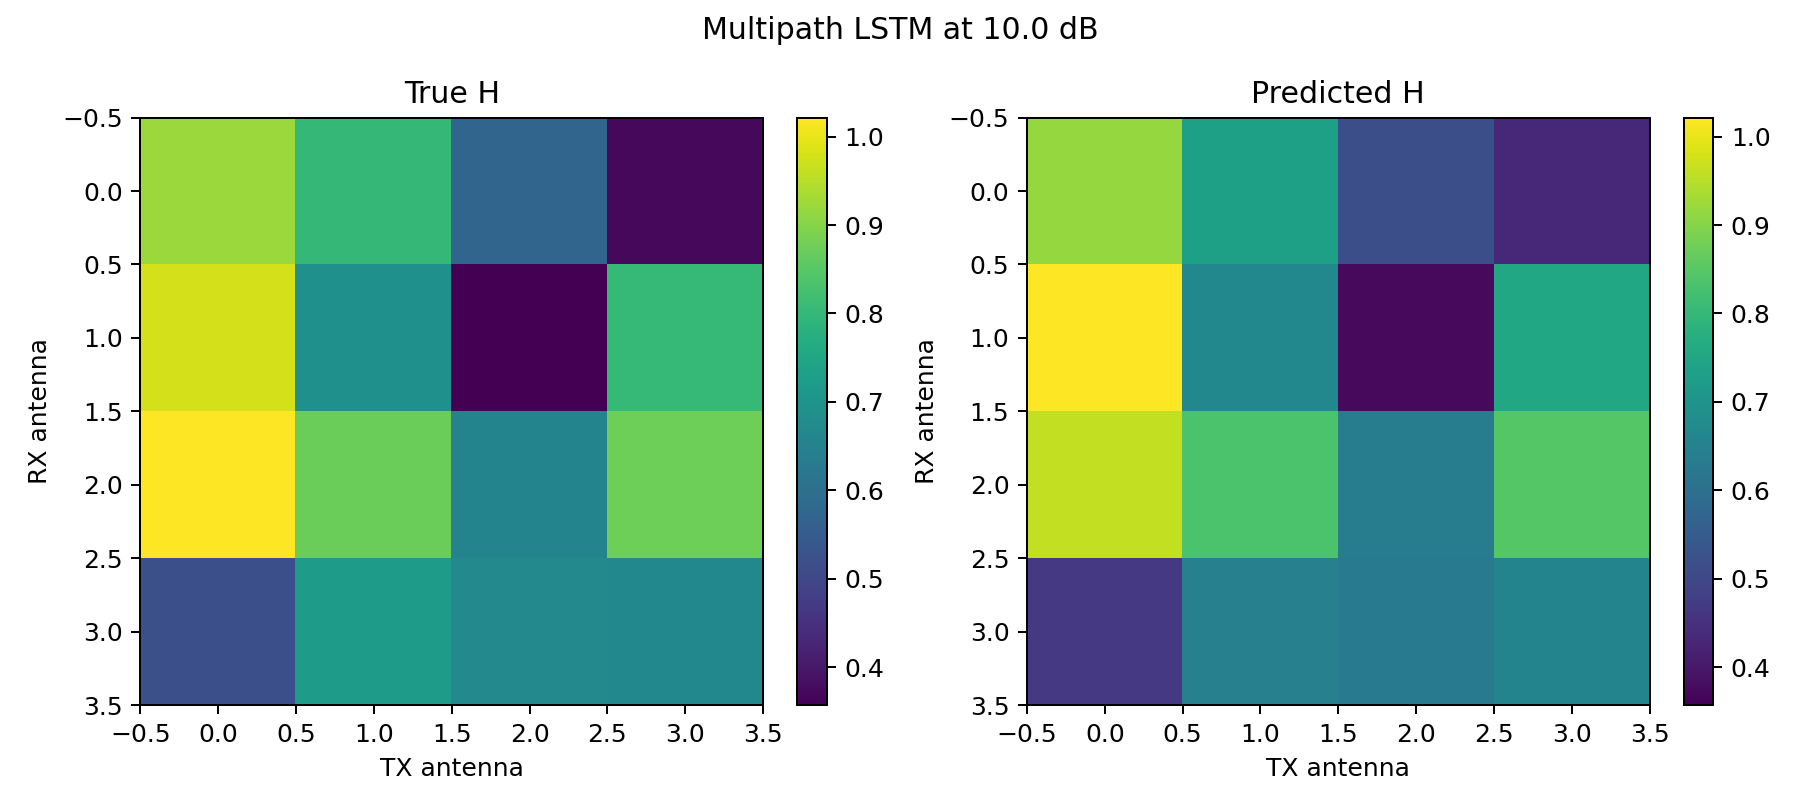
\includegraphics[width=\linewidth]{Multipath_lstm_Heatmap.png}
    \caption{LSTM}
  \end{subfigure}\hfill
  \begin{subfigure}[t]{0.32\textwidth}
    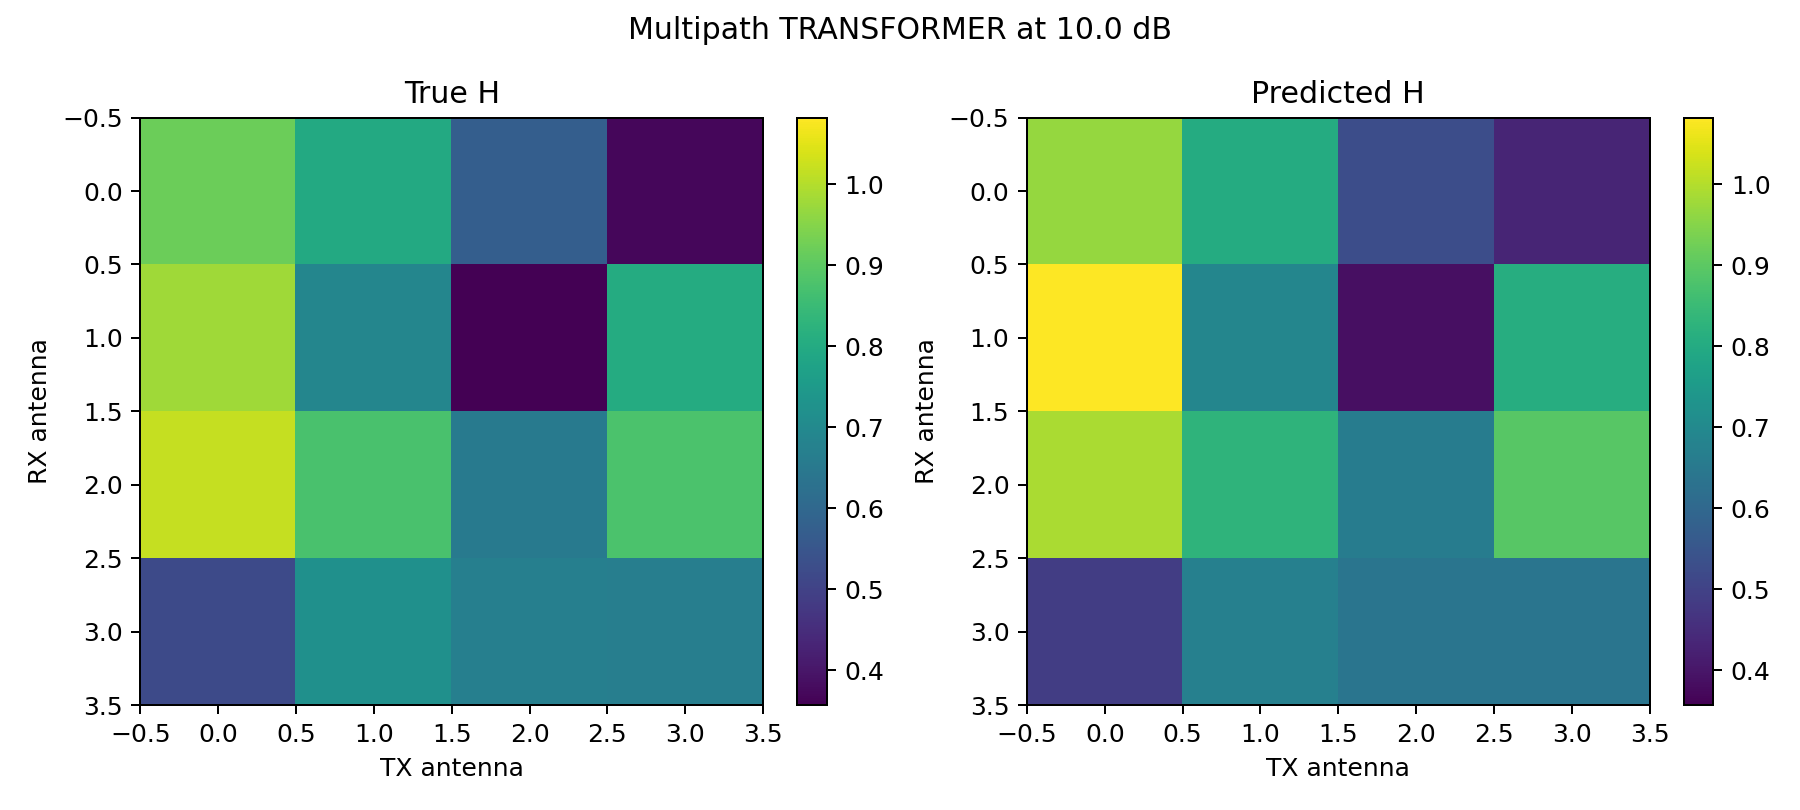
\includegraphics[width=\linewidth]{Multipath_transformer_Heatmap.png}
    \caption{Transformer}
  \end{subfigure}
  \caption{相关多径信道在约 10 dB 时的真实幅度与预测幅度}
  \label{fig:multipath_heat}
\end{figure}

图~\ref{fig:multipath_residual} 中残差均围绕零对称，CNN 的分布中心最尖锐、尾部收缩最明显，Transformer 次之，LSTM 相对更宽；这一顺序与该场景下 $-15.06$、$-14.08$、$-12.67$ dB 的测试 NMSE 相符。因此，损失曲线、单样本重构图和全测试集残差统计三类证据相互支持：相关多径结构确实为深度估计带来了可重复利用的信息。

\begin{figure}[H]
  \centering
  \begin{subfigure}[t]{0.32\textwidth}
    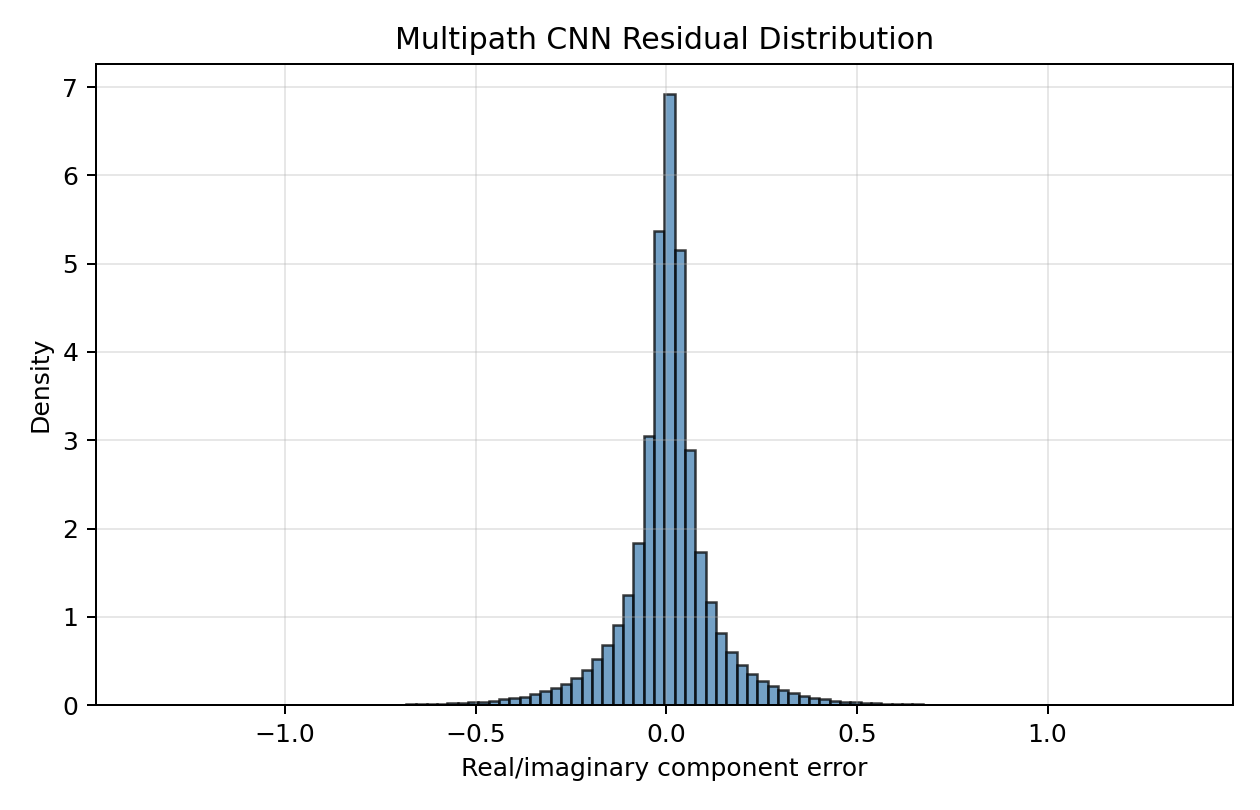
\includegraphics[width=\linewidth]{Multipath_cnn_ResidualHistogram.png}
    \caption{CNN}
  \end{subfigure}\hfill
  \begin{subfigure}[t]{0.32\textwidth}
    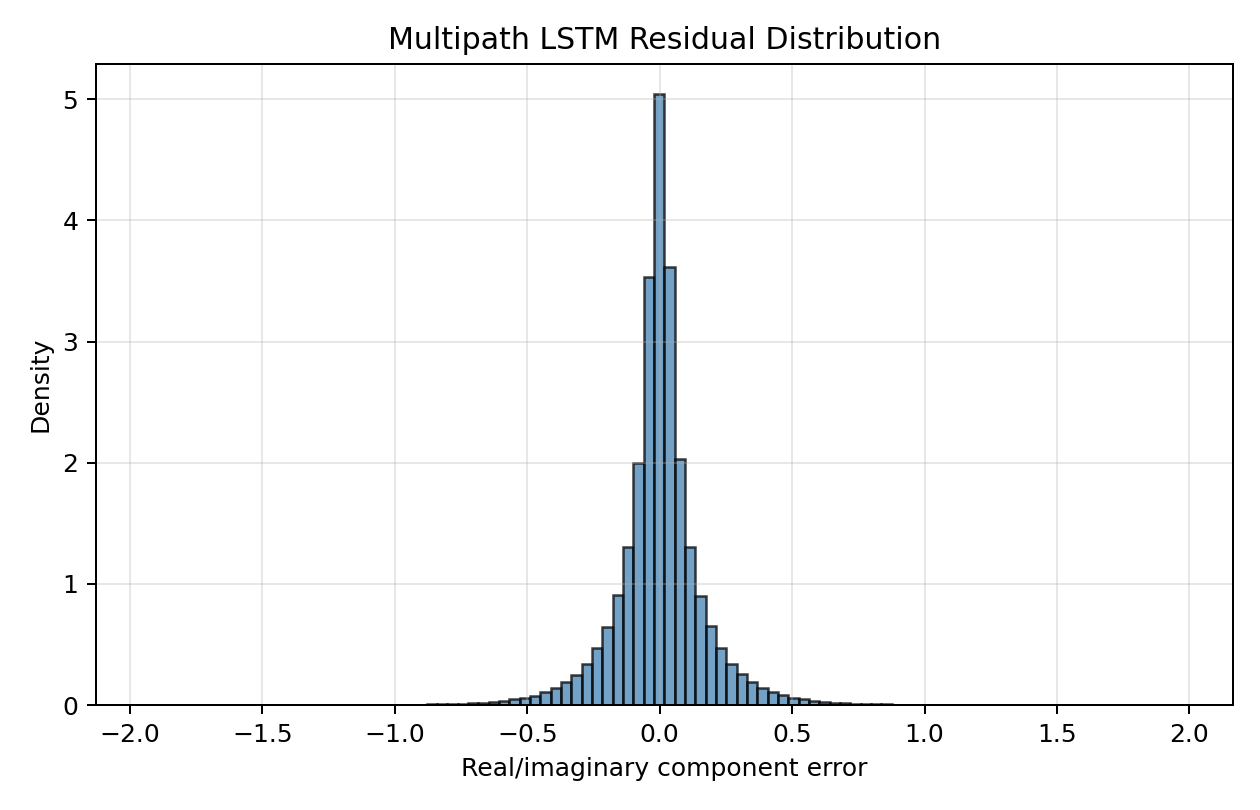
\includegraphics[width=\linewidth]{Multipath_lstm_ResidualHistogram.png}
    \caption{LSTM}
  \end{subfigure}\hfill
  \begin{subfigure}[t]{0.32\textwidth}
    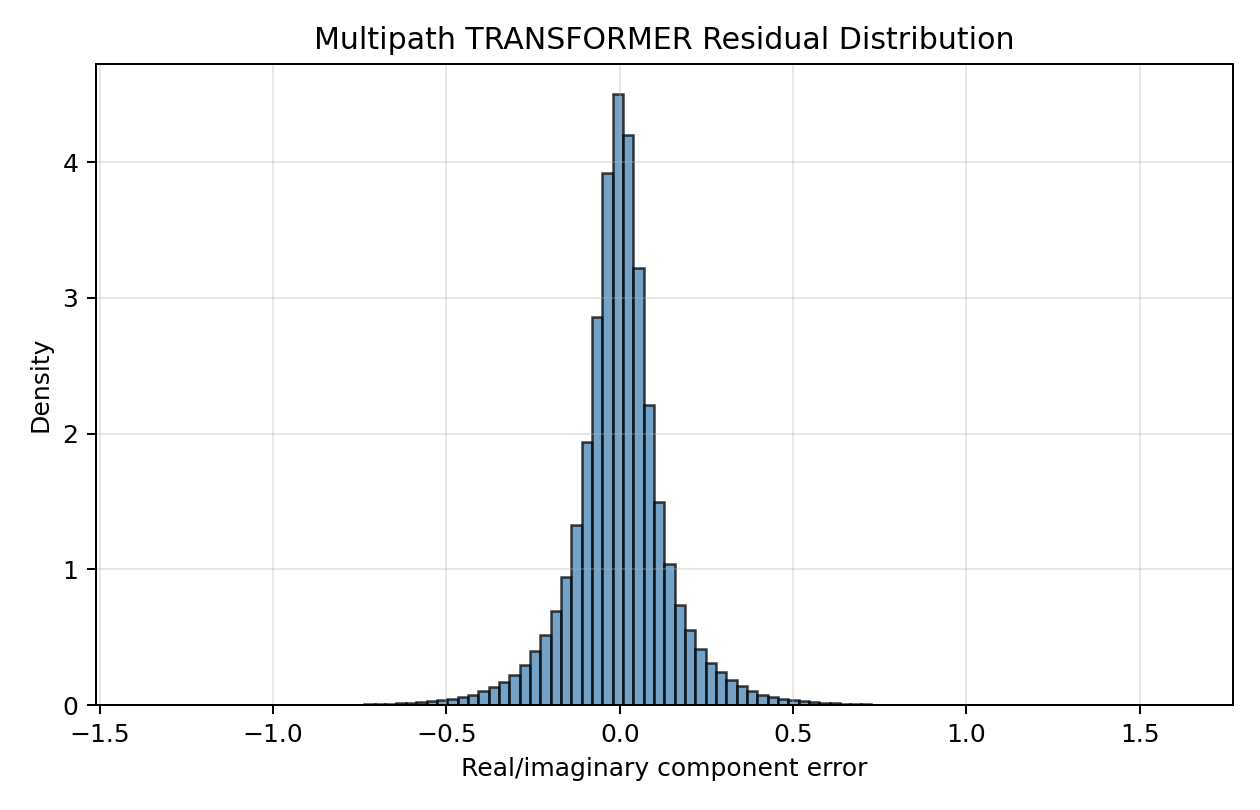
\includegraphics[width=\linewidth]{Multipath_transformer_ResidualHistogram.png}
    \caption{Transformer}
  \end{subfigure}
  \caption{相关多径信道下三种网络的实部/虚部残差分布}
  \label{fig:multipath_residual}
\end{figure}

\section{改进与提高}

在基础 CNN、LSTM 与 Transformer 对比完成后，本实验进一步从“增加网络表达能力”和“引入无线信道物理先验”两条路线进行提高。前者构造增强残差 CNN，检验单纯加深网络是否足以继续降低误差；后者将有限时延扩展约束显式嵌入估计流程，检验模型驱动与数据驱动相结合的收益。

\subsection{增强残差 CNN}

原始 CNN 仅包含两层 $3\times3\times3$ 卷积和一层 $1\times1\times1$ 输出卷积，共 30,370 个参数。增强 CNN 将隐藏通道数提高到 48，并串联 4 个三维残差块；每个残差块使用两层卷积、GroupNorm 与 SiLU 激活。其输入同时包含 LS、标量 LMMSE 和对数噪声方差，并以 LMMSE 为残差学习起点：
\begin{equation}
  \widehat{\bm H}_{\mathrm{enh}}
  =\widehat{\bm H}_{\mathrm{LMMSE}}+
  f_{\theta}\!\left(\widehat{\bm H}_{\mathrm{LS}},
  \widehat{\bm H}_{\mathrm{LMMSE}},\log_{10}\sigma_n^2\right).
\end{equation}
增强模型参数量为 505,538，是原始 CNN 的约 16.65 倍。二者使用相同数据、随机种子和训练预算，以保证比较公平。

\begin{table}[H]
  \centering
  \caption{原始 CNN 与增强残差 CNN 的提高实验}
  \label{tab:improved_cnn}
  \begin{tabular}{lrrr}
    \toprule
    模型 & 测试 NMSE (dB) & 参数量 & 最优验证 NMSE \\
    \midrule
    原始 CNN & $-14.9181$ & 30,370 & 0.027057 \\
    增强 CNN & $-14.9852$ & 505,538 & 0.026998 \\
    \bottomrule
  \end{tabular}
\end{table}

\begin{figure}[H]
  \centering
  \begin{subfigure}[t]{0.49\textwidth}
    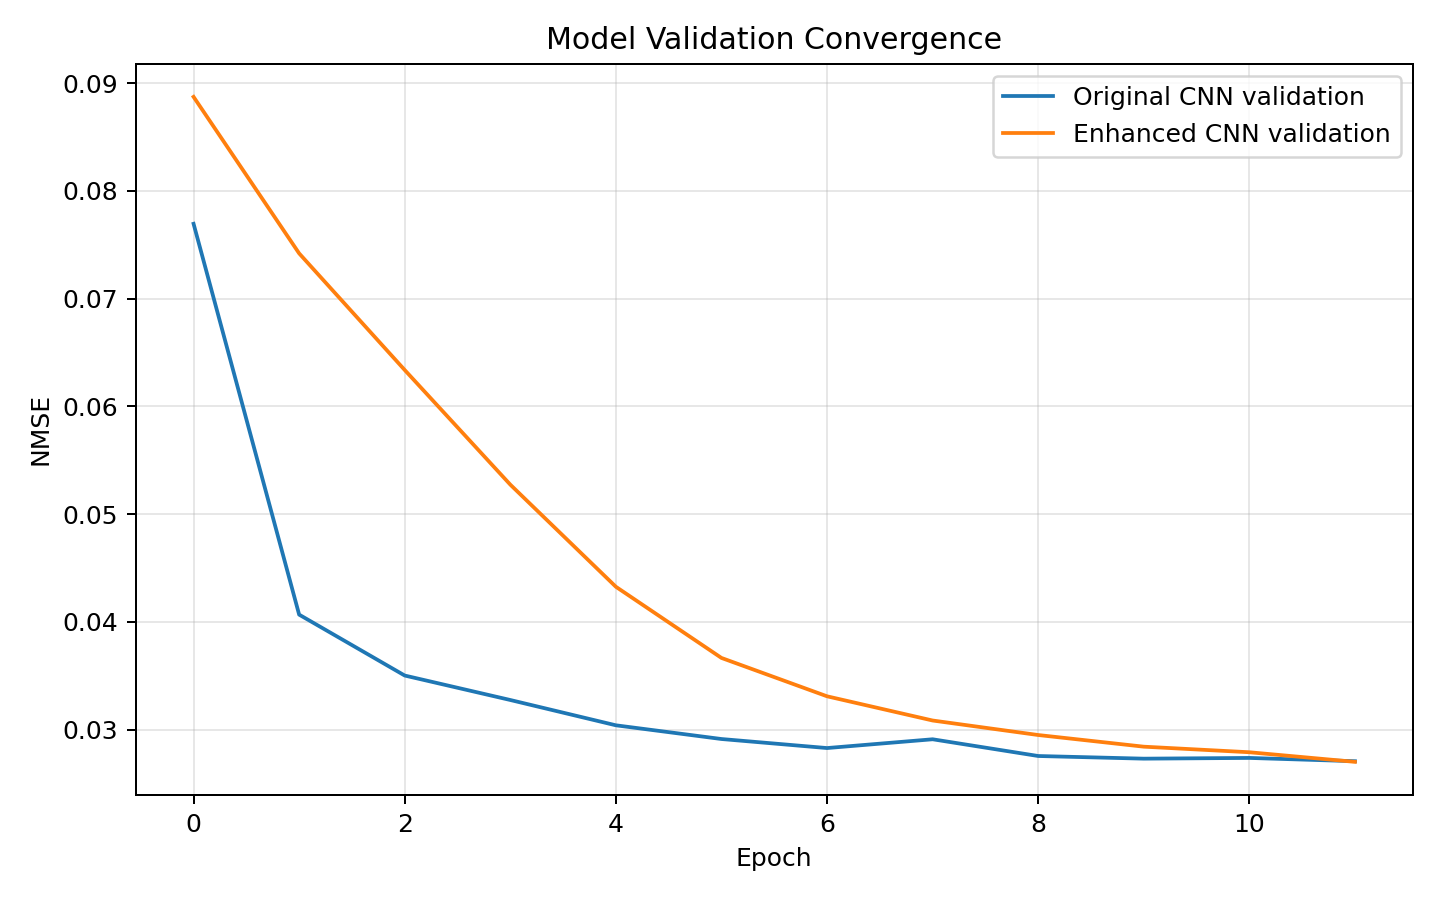
\includegraphics[width=\linewidth]{improved/improved_convergence.png}
    \caption{验证集收敛曲线}
  \end{subfigure}\hfill
  \begin{subfigure}[t]{0.49\textwidth}
    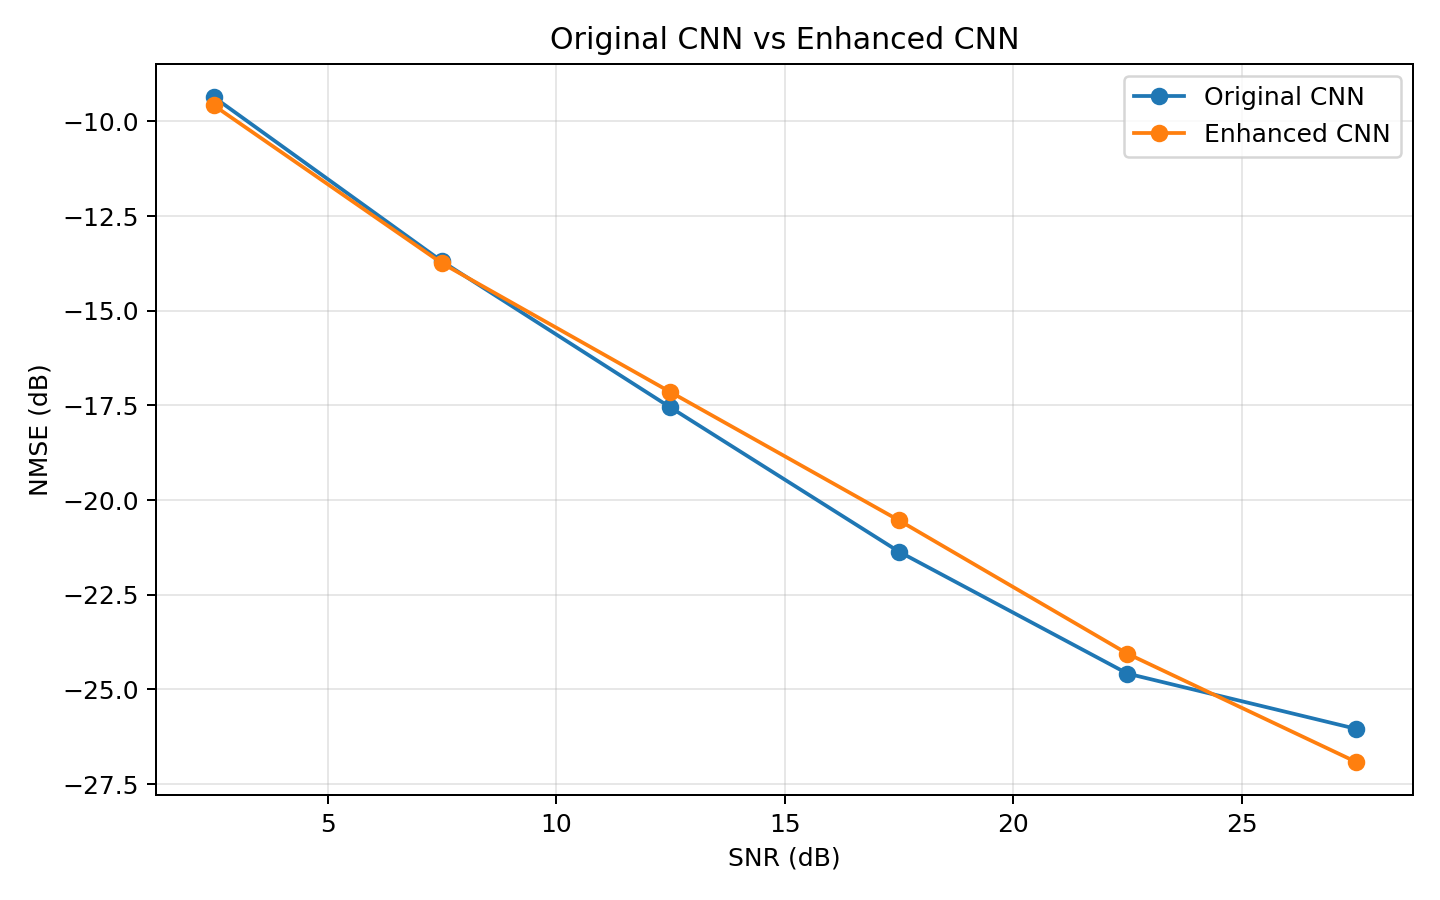
\includegraphics[width=\linewidth]{improved/improved_nmse_vs_snr.png}
    \caption{不同 SNR 区间的 NMSE}
  \end{subfigure}
  \caption{原始 CNN 与增强残差 CNN 的收敛及分 SNR 性能}
  \label{fig:improved_curves}
\end{figure}

图~\ref{fig:improved_curves}(a) 显示，原始 CNN 在训练初期收敛更快，而增强 CNN 经过约 10 轮后才追平；最终两者验证 NMSE 几乎相同。图~\ref{fig:improved_curves}(b) 表明增强 CNN 只在最低和最高 SNR 区间略占优势，在中间区间反而轻微落后。总体测试 NMSE 仅改善 0.067 dB，却付出了 16.65 倍参数量，因此单纯增加深度和宽度没有带来与复杂度相称的收益。该负面结果同样有价值：当前任务的瓶颈并非网络容量不足，而更可能是如何有效利用已知信道结构。

图~\ref{fig:improved_heatmaps} 中两种模型均能保持真实信道的主要空间幅度模式，视觉差异很小；图~\ref{fig:improved_residuals} 中两者相对 LS/LMMSE 都显著压缩了残差，但增强模型并未形成明显更窄的整体分布。这与表~\ref{tab:improved_cnn} 的微小数值差距相互印证。

\begin{figure}[H]
  \centering
  \begin{subfigure}[t]{0.49\textwidth}
    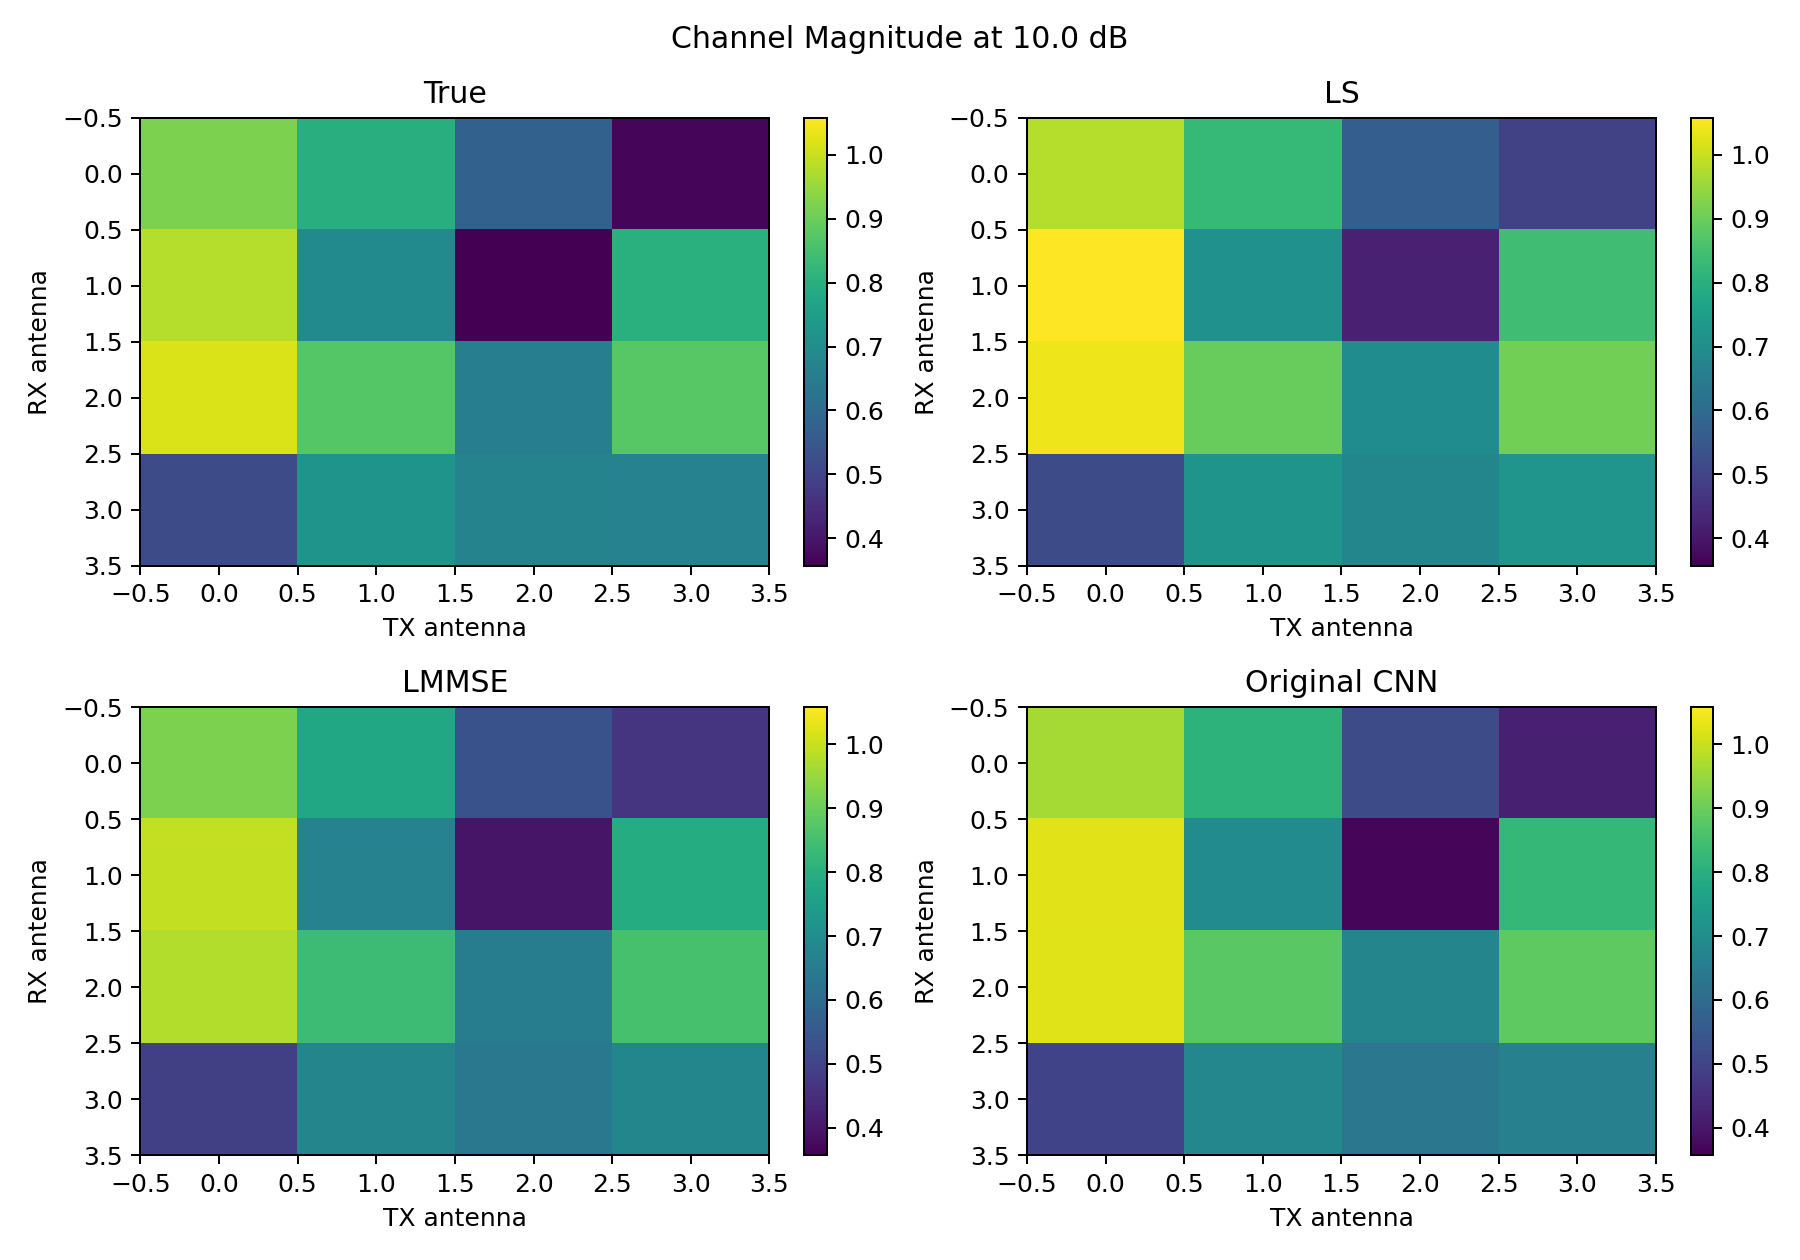
\includegraphics[width=\linewidth]{improved/original_cnn_heatmap.png}
    \caption{原始 CNN}
  \end{subfigure}\hfill
  \begin{subfigure}[t]{0.49\textwidth}
    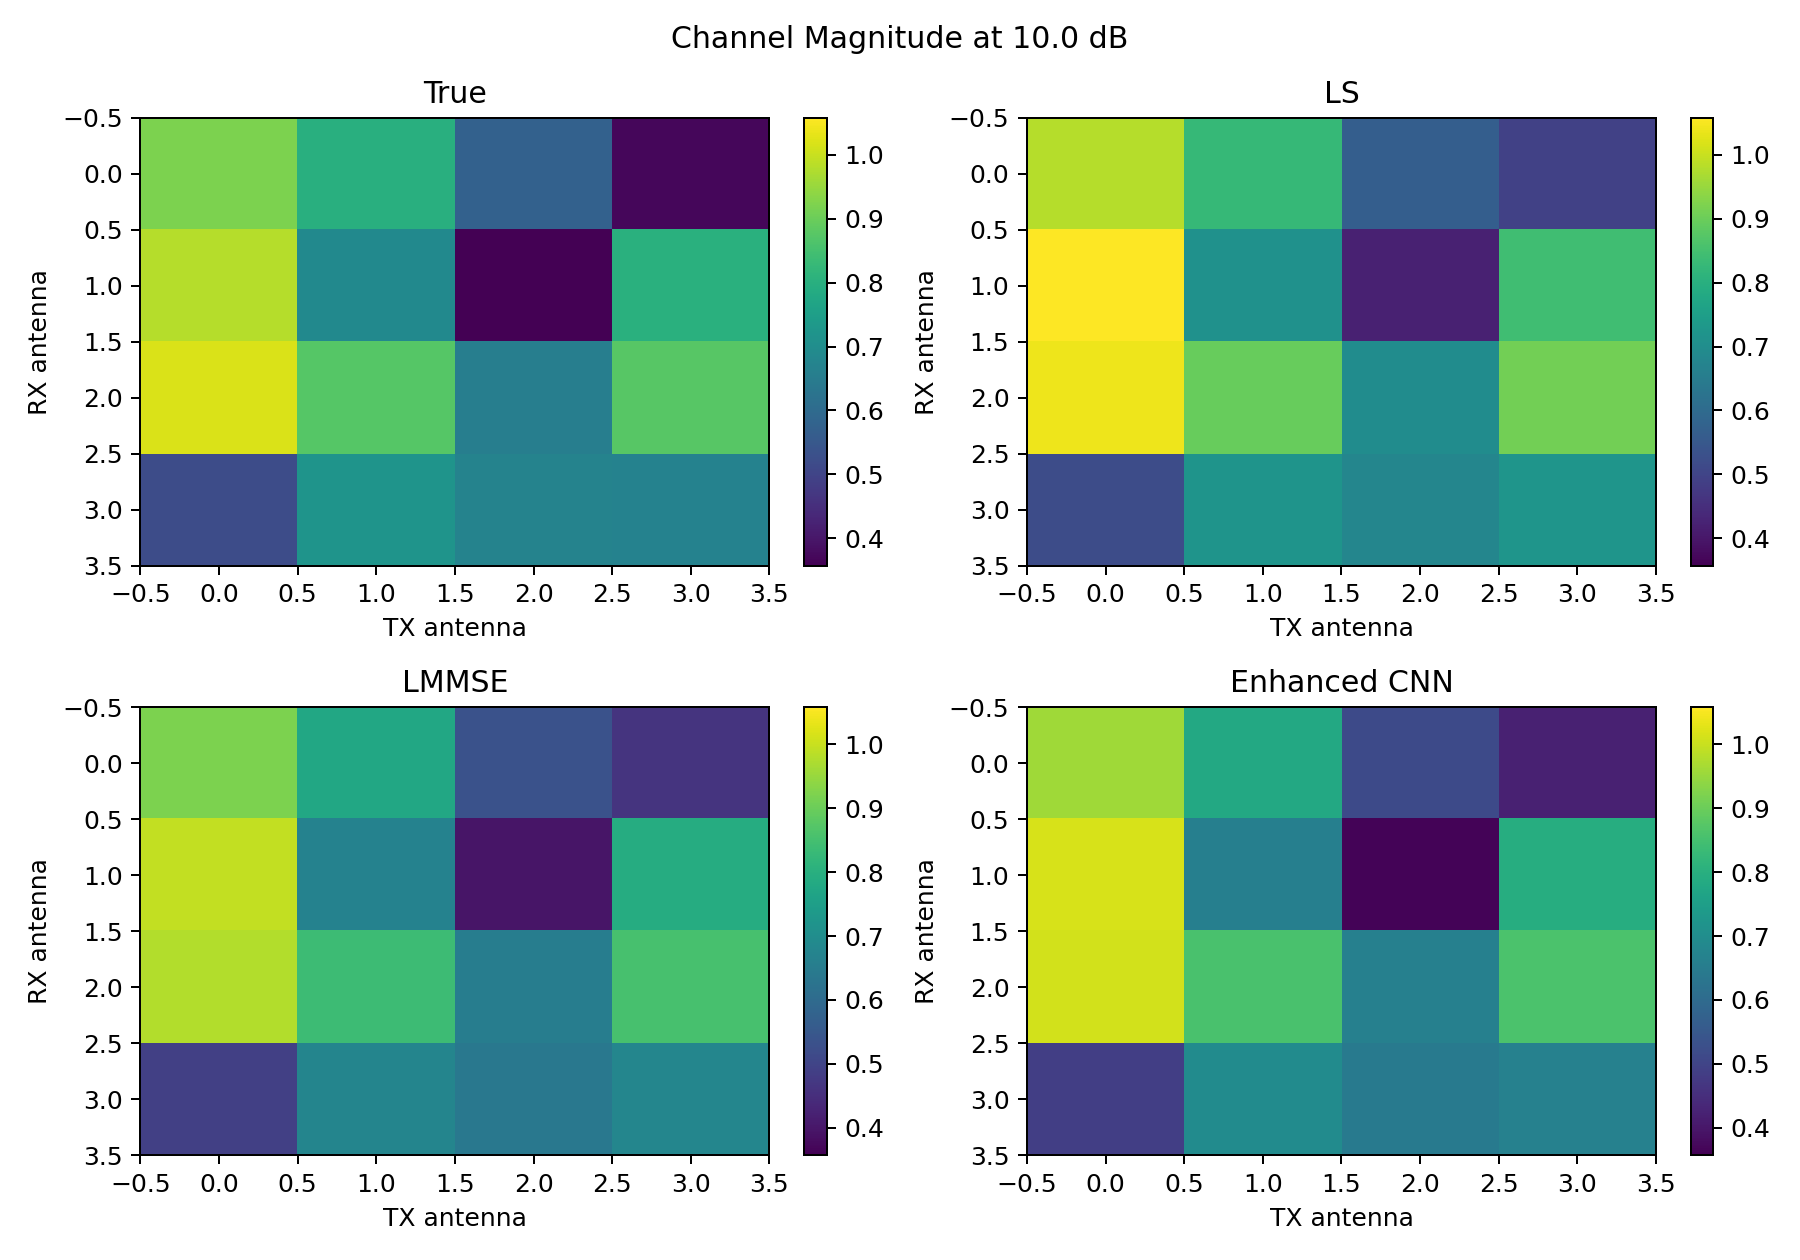
\includegraphics[width=\linewidth]{improved/enhanced_cnn_heatmap.png}
    \caption{增强 CNN}
  \end{subfigure}
  \caption{原始与增强 CNN 的统一四联信道幅度诊断}
  \label{fig:improved_heatmaps}
\end{figure}

\begin{figure}[H]
  \centering
  \begin{subfigure}[t]{0.49\textwidth}
    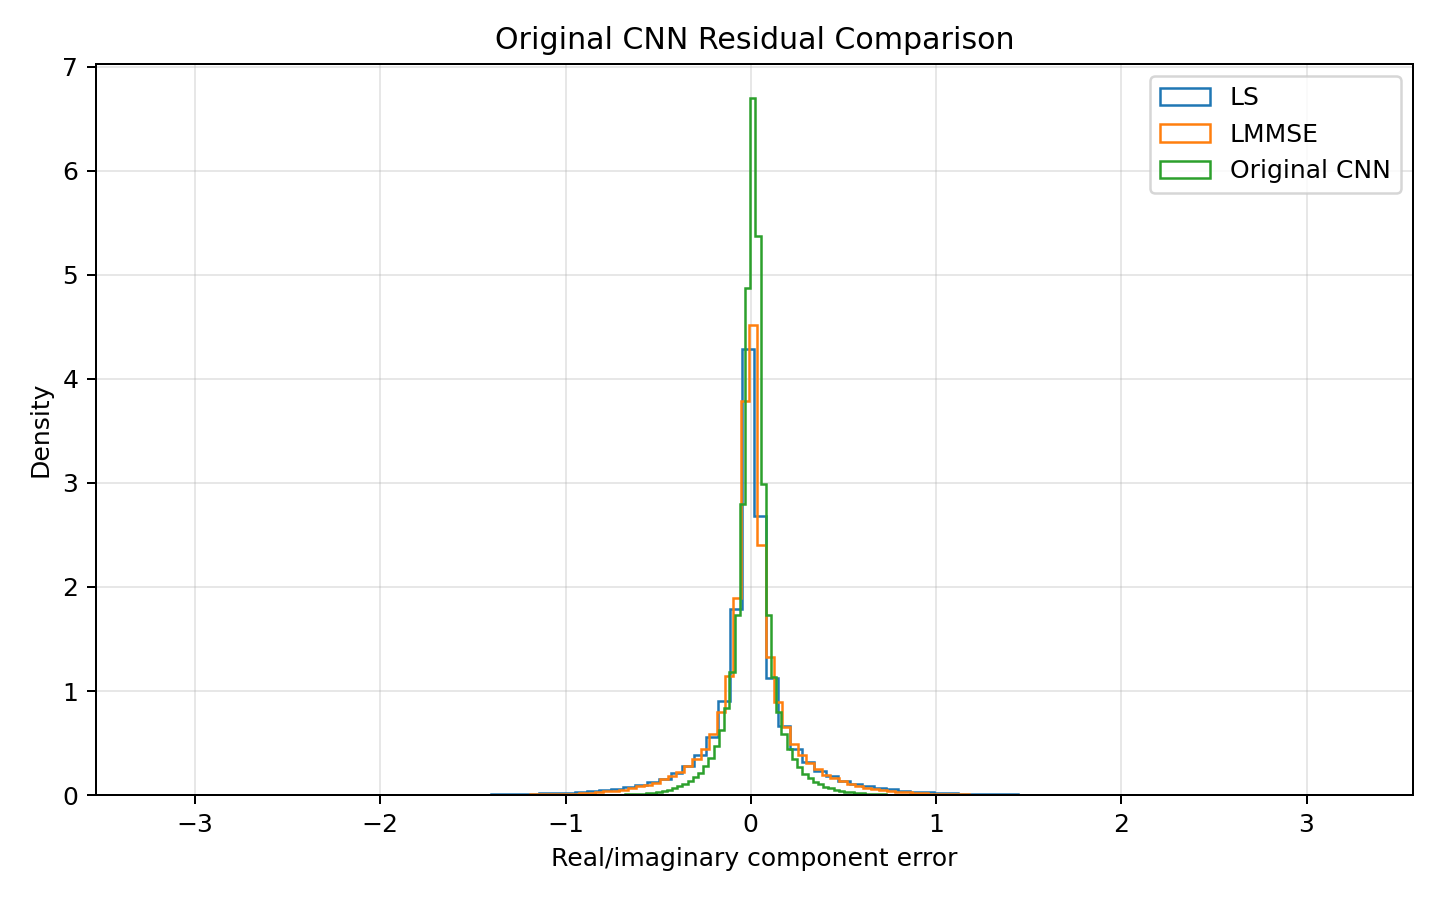
\includegraphics[width=\linewidth]{improved/original_cnn_residual.png}
    \caption{原始 CNN}
  \end{subfigure}\hfill
  \begin{subfigure}[t]{0.49\textwidth}
    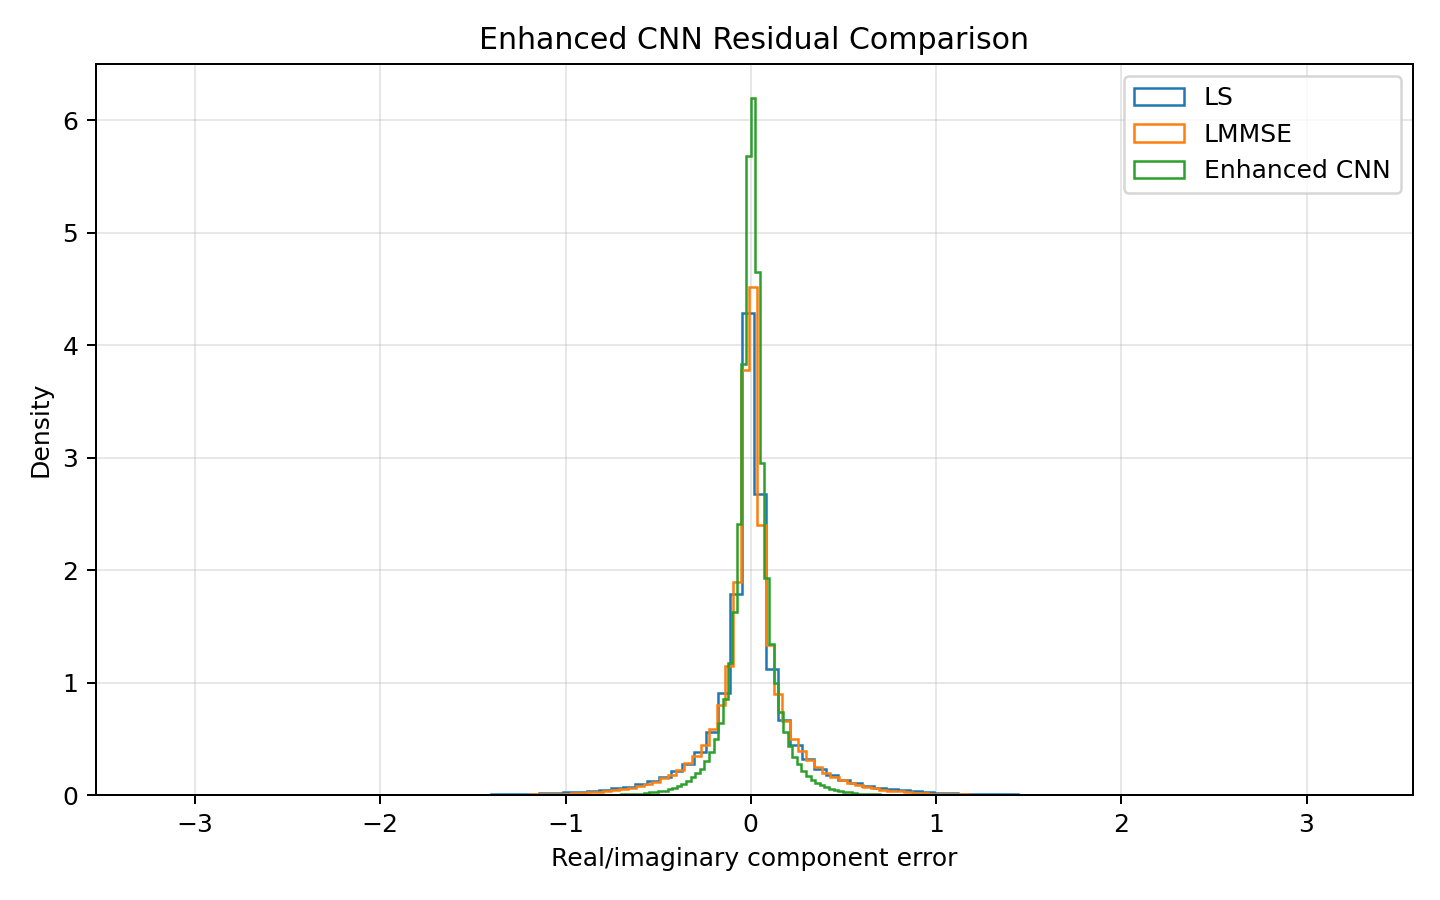
\includegraphics[width=\linewidth]{improved/enhanced_cnn_residual.png}
    \caption{增强 CNN}
  \end{subfigure}
  \caption{原始与增强 CNN 相对传统基线的残差分布}
  \label{fig:improved_residuals}
\end{figure}

\subsection{基于有限时延扩展的物理引导提高}

合成多径信道由 $L=6$ 条时域径生成，因此其理想信道冲激响应在第 6 个抽头之后为零。利用这一先验，可将任意频域估计 $\widehat{\bm H}$ 先变换到时域、截断超出最大时延的抽头，再变回频域：
\begin{equation}
  \mathcal P_L(\widehat{\bm H})
  =\operatorname{FFT}\!\left(
    \bm M_L\odot\operatorname{IFFT}(\widehat{\bm H})
  \right),
\end{equation}
其中 $\bm M_L$ 在前 $L$ 个抽头处为 1，其余位置为 0。该投影直接滤除了不符合有限时延模型的噪声分量。

进一步构造的 Physics-Guided CNN 同时接收 LS、LMMSE、LS 的时延投影以及噪声特征，以投影结果为残差起点，并在网络输出端再次执行 $\mathcal P_L$，从结构上保证最终估计满足已知最大时延约束。

\begin{table}[H]
  \centering
  \caption{物理引导提高方法的测试 NMSE（dB）}
  \label{tab:physics}
  \begin{tabular}{lr@{\hspace{1cm}}lr}
    \toprule
    方法 & NMSE & 方法 & NMSE \\
    \midrule
    LS & $-8.2665$ & LS + 时延投影 & $-15.5632$ \\
    LMMSE & $-9.8111$ & LMMSE + 时延投影 & $-13.6035$ \\
    CNN & $-14.9181$ & CNN + 时延投影 & $-16.7841$ \\
    \multicolumn{3}{l}{Physics-Guided CNN} & $\mathbf{-17.1401}$ \\
    \bottomrule
  \end{tabular}
\end{table}

\begin{figure}[H]
  \centering
  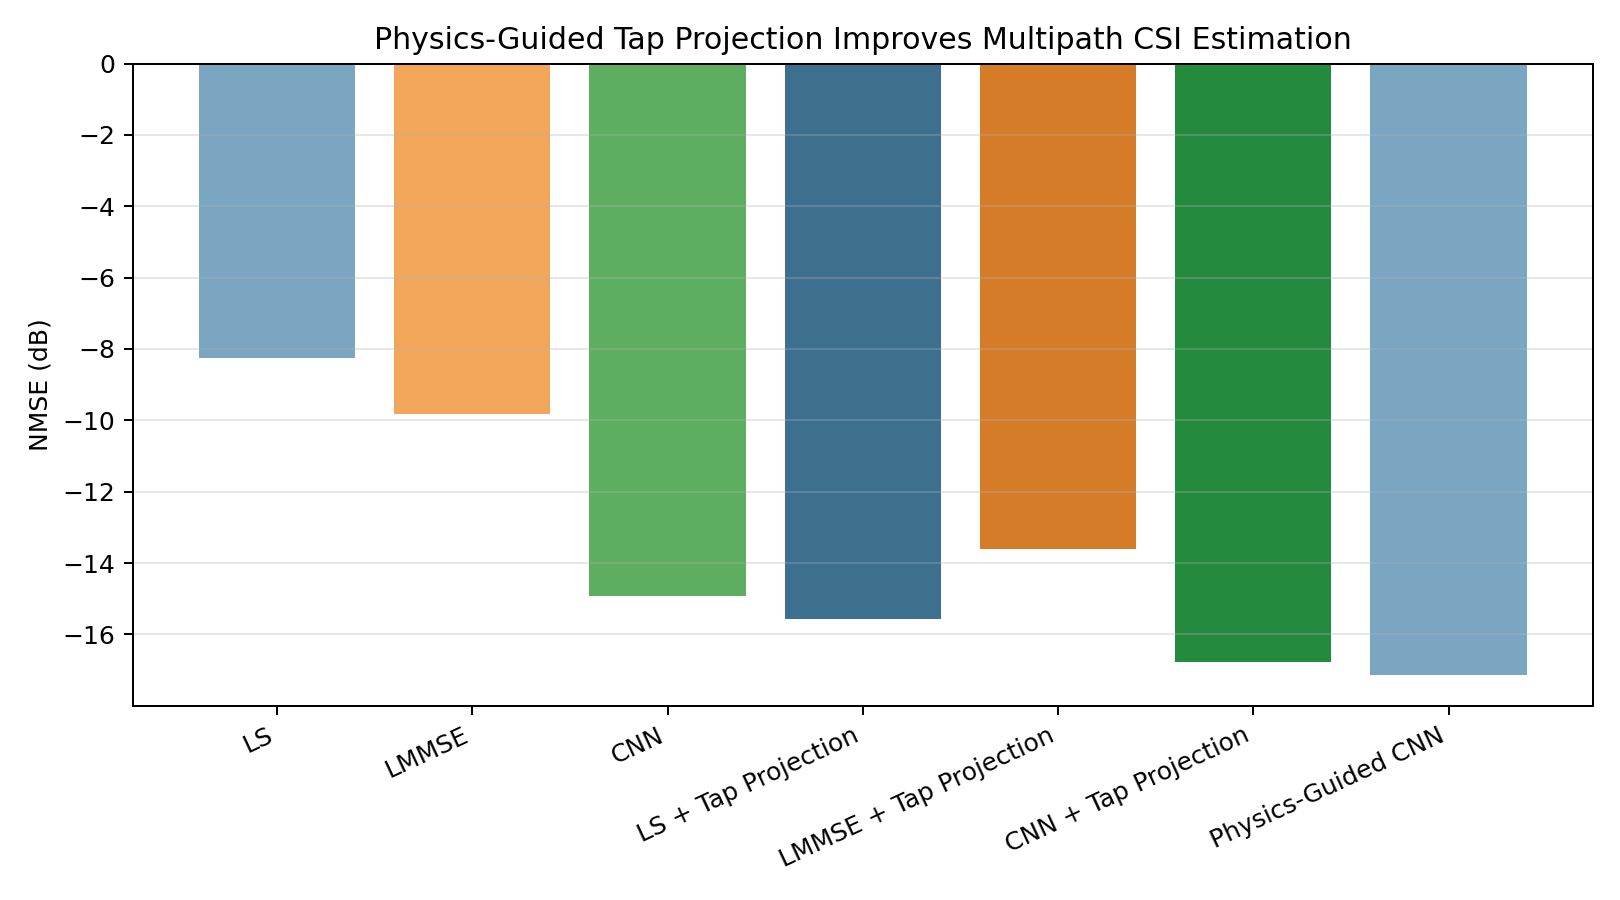
\includegraphics[width=0.88\textwidth]{physics_guided/physics_guided_bar.png}
  \caption{传统估计、后处理投影与物理引导 CNN 的总体 NMSE 对比}
  \label{fig:physics_bar}
\end{figure}

表~\ref{tab:physics} 与图~\ref{fig:physics_bar} 显示，LS 经过时延投影后提高 7.30 dB，甚至超过未经投影的 CNN；CNN 加投影比原始 CNN 提高 1.87 dB。Physics-Guided CNN 达到 $-17.14$ dB，相对原始 CNN 提高 2.22 dB，相对标量 LMMSE 提高 7.33 dB，并比简单的 CNN 后处理投影再提高 0.36 dB。相比增强 CNN 仅 0.067 dB 的增益，物理先验带来的收益更显著，说明“正确的归纳偏置”比单纯堆叠参数更有效。

\begin{figure}[H]
  \centering
  \begin{subfigure}[t]{0.49\textwidth}
    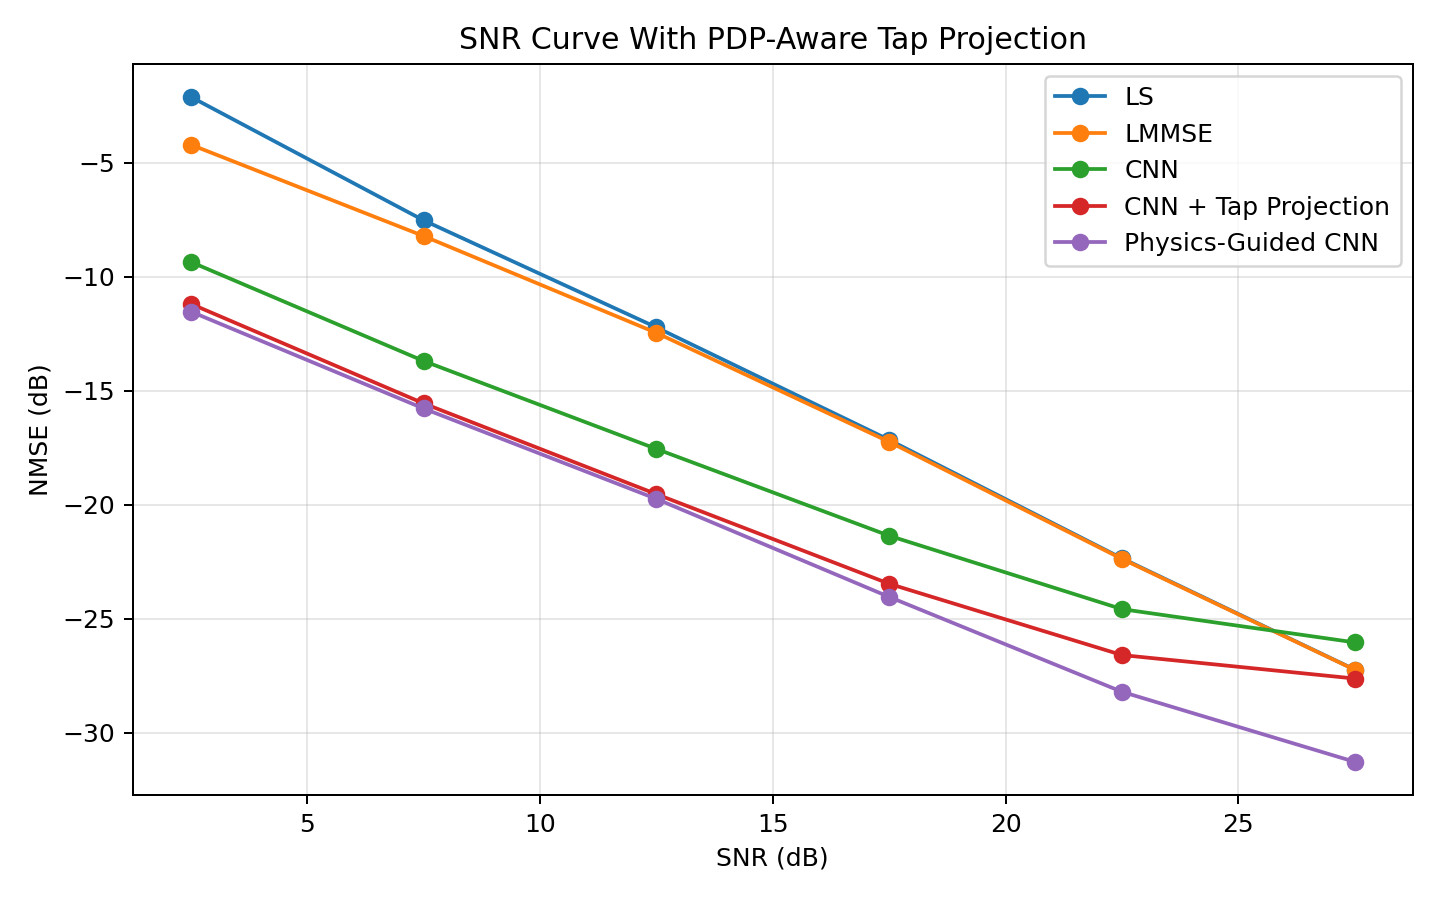
\includegraphics[width=\linewidth]{physics_guided/physics_guided_snr.png}
    \caption{不同 SNR 区间的性能}
  \end{subfigure}\hfill
  \begin{subfigure}[t]{0.49\textwidth}
    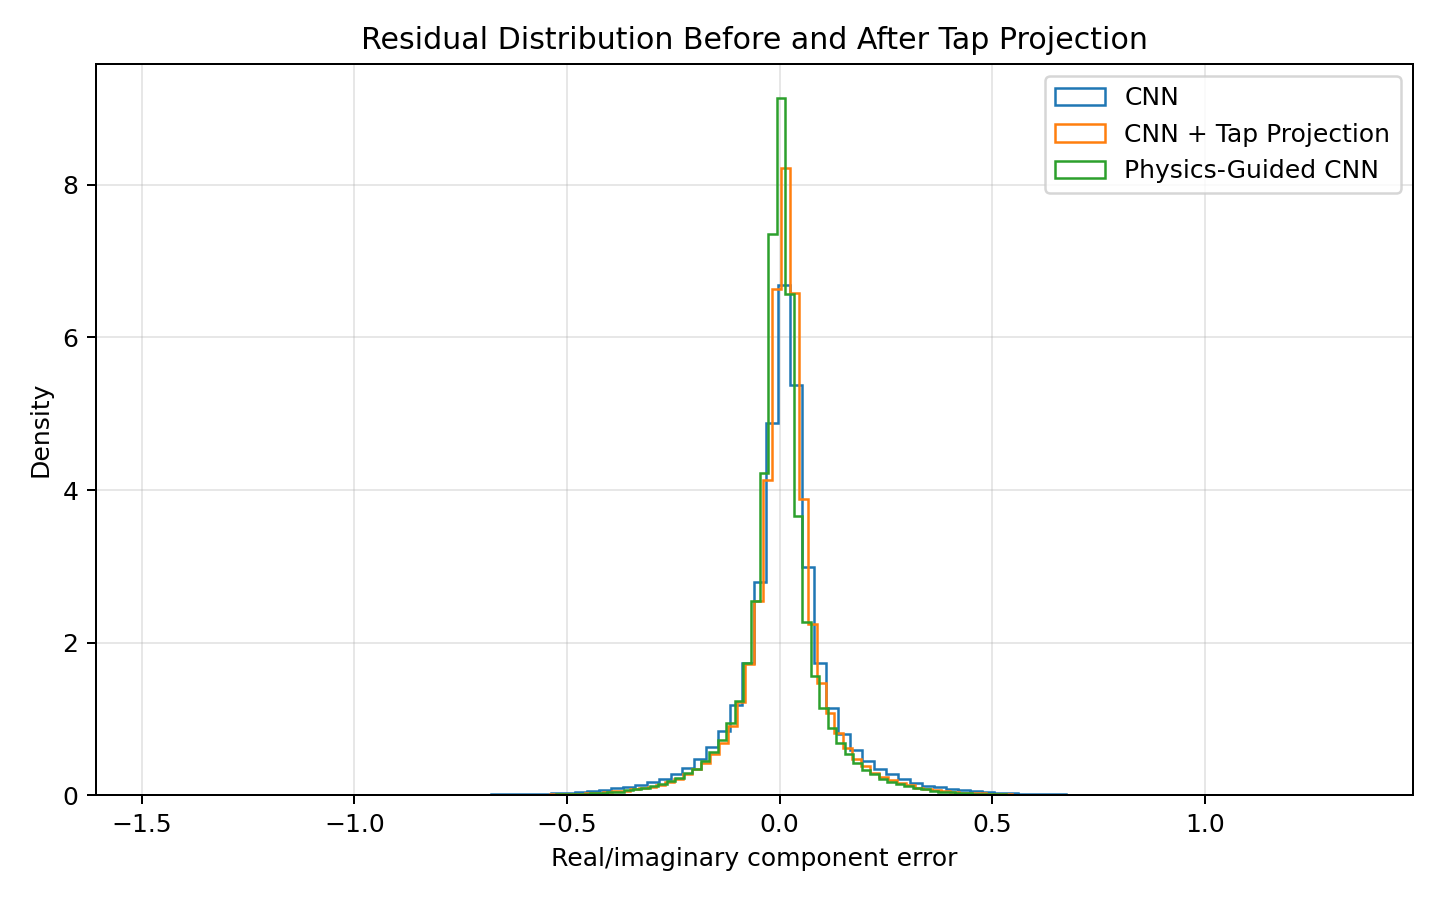
\includegraphics[width=\linewidth]{physics_guided/physics_guided_residual.png}
    \caption{投影前后的残差分布}
  \end{subfigure}
  \caption{物理引导时延投影的分 SNR 性能与残差诊断}
  \label{fig:physics_diagnostics}
\end{figure}

图~\ref{fig:physics_diagnostics}(a) 中，CNN 加投影和 Physics-Guided CNN 在全部 SNR 区间均优于原始 CNN，且物理引导模型在高 SNR 处仍持续下降，没有出现原始 CNN 那样明显的误差地板。图~\ref{fig:physics_diagnostics}(b) 中，物理引导模型的残差中心峰最高、分布最集中，再次验证了其定量优势。

需要强调的是，本实验的最大时延 $L=6$ 与数据生成模型完全匹配，属于理想先验条件。实际系统中的时延扩展可能随场景变化，并受同步误差和循环前缀配置影响；若先验 $L$ 设置过小，会截断真实有效路径并造成偏差。因此，该提高结果证明了物理引导思想的有效性，但真实部署时应通过信道测量或自适应机制确定时延窗口。

\section{讨论与实验局限}

\begin{enumerate}[label=(\arabic*)]
  \item \textbf{LMMSE 基线范围：} 本实验使用式~\eqref{eq:lmmse} 的标量 LMMSE，并未显式利用真实空频协方差。若采用协方差感知的矩阵 LMMSE，相关多径场景下的传统基线预计会更强。
  \item \textbf{数据真实性：} 所有结果均来自合成信道，不能直接表述为真实无线环境或 DeepMIMO 数据集上的结论。硬件非理想、导频同步误差和信道分布偏移仍需实测验证。
  \item \textbf{单次运行波动：} 当前结果基于给定随机种子的单次训练。架构绝对排名在不同独立运行间出现变化，严谨比较应使用多个随机种子并报告均值与置信区间。
  \item \textbf{复杂度评价：} 已统计参数量，但现有图片未给出统一硬件上的推理时延与显存占用。因此本文只对模型规模进行分析，不对实时性作未经测量的结论。
  \item \textbf{高 SNR 误差地板：} CNN 在 30 dB 时略逊于解析基线，后续可引入恒等映射门控，使模型在噪声极小时自适应退化为 LS/LMMSE。
  \item \textbf{物理先验匹配：} 时延投影使用了与合成数据完全一致的 6 径上限，结果代表先验准确时的性能上界；仍需补充时延窗口失配实验，以评价模型对未知或变化时延扩展的鲁棒性。
\end{enumerate}

\section{结论}

本实验完成了从 MIMO--OFDM 信道生成、正交导频观测、传统估计到深度残差估计的完整流程，并利用独立测试集进行了统一评价。主要结论如下：

\begin{enumerate}[label=(\arabic*)]
  \item CNN 在中低 SNR 的相关多径信道上显著优于 LS 和标量 LMMSE，10 dB 时相对 LMMSE 改善约 5.62 dB；
  \item 混合 SNR 架构对比中 Transformer 的总体精度最高，而 CNN 仅用 30,370 个参数取得接近的性能，是更有吸引力的轻量化方案；
  \item 深度模型在独立 Rayleigh 信道上没有明显优势，在相关多径信道上才获得 2.86--5.25 dB 增益，表明学习方法依赖可利用的空频结构；
  \item 可视化结果与 NMSE 指标相互印证，网络能够恢复主要信道幅度结构并使残差更集中于零；
  \item 当前结论适用于给定合成模型与标量 LMMSE 基线。多随机种子、全协方差 LMMSE 和实测信道验证是下一阶段工作的重点。
  \item 新增提高实验表明，增强 CNN 以 16.65 倍参数量仅换取 0.067 dB 改善，而 Physics-Guided CNN 相对原始 CNN 提高 2.22 dB；在本任务中，引入正确的有限时延物理先验比单纯扩大网络更有效。
\end{enumerate}

\appendix
\section{复现实验}

在项目根目录激活环境后，可运行完整实验：
\begin{lstlisting}[language={}]
.\gpu-env\.venv\Scripts\Activate.ps1
python run_complete_experiments.py --device cuda
\end{lstlisting}

本文仅将 \path{results/complete} 中的 36 张正式实验图片用于结果分析，并已全部纳入正文。其余带有 \path{smoke} 或 \path{cleanup_check} 标记的目录属于快速通路检查或清理验证结果；其中 quick 模式仅使用 512/128/256 个训练/验证/测试样本并训练 2 轮，程序说明明确规定其精度不能作为最终实验结论，故不与正式结果混用。

核心结果分别保存在：
\begin{itemize}
  \item \texttt{results/complete/snr/metrics.json}：固定 SNR 对比；
  \item \texttt{results/complete/models/metrics.json}：模型总体性能与参数量；
  \item \texttt{results/complete/figure\_matrix\_metrics.json}：信道场景消融；
  \item \texttt{results/complete/}：本文引用的全部实验图片。
\end{itemize}

报告使用 XeLaTeX 编译：
\begin{lstlisting}[language={}]
xelatex report.tex
xelatex report.tex
\end{lstlisting}

\end{document}
